\subsection{D(A) 上的幺半群结构}

命题 3. 设 \(\mathfrak{a}, \mathfrak{a}', \mathfrak{b}, \mathfrak{b}'\) 是 I(A) 中的元素。关系 \(\mathfrak{a} > \mathfrak{a}'\) 和 \(\mathfrak{b} > \mathfrak{b}'\) 蕴含 \(\mathfrak{ab} > \mathfrak{a}'\mathfrak{b}'\)。

我们可以把注意力限制在 \(\mathfrak{b} = \mathfrak{b}'\) 的情形。令 \(Ax\) 为包含 \(a'b\) 的分式主理想；对于每个非零元 \(y\)（\(\mathfrak{b}\) 中的），有 \(Ax \supset a'y\)，从而 \(Axy^{-1} \supset a'\)，于是 \(Axy^{-1} \supset a\) 且 \(Ax \supset ay\)。让 \(y\) 变化可见 \(Ax \supset ab\)，因此 \(ab > a'b\)。

由命题 3 可知，I(A) 上的乘法通过取商在 D(A) 上定义了一个合成律，该合成律显然满足结合律和交换律。我们采用加法记号，从而可以写成：

\[
\operatorname{div} (a b) = \operatorname{div} a + \operatorname{div} b,\tag{2}
\]

其中 a, b 属于 I(A)。显然 div(1) 是这个加法的单位元；将此元素记作 0。命题 3 进一步证明，D(A) 上的序结构与这个加法相容（《代数》第 VI 章，§ 1，第 1 节），更精确地说（第 1 节，命题 2 (ii)）：

\[
\begin{array}{r l} \inf (\operatorname{div} a + \operatorname{div} b, \operatorname{div} a + \operatorname{div} c) & = \inf (\operatorname{div} (a b), \operatorname{div} (a c)) = \operatorname{div} (a b + a c) \\ & = \operatorname{div} (a (b + c)) = \operatorname{div} a + \operatorname{div} (b + c) = \operatorname{div} a + \inf (\operatorname{div} b, \operatorname{div} c). \end{array}
\]

对于分式理想 \(a \neq 0\)，要使其在 D(A) 中满足 div \(a \geqslant 0\)，充要条件是 \(a \subset A\)（换句话说，a 是 A 的整理想）。

对于两个元素 \(x, y\)（属于 \(\mathbf{K}^*\)），关系 \(\operatorname{div}(x) = \operatorname{div}(y)\) 等价于 \(A x = A y\)；\(A\) 的主除子集合（带有由 \(D(A)\) 诱导的序关系和幺半群运算）是一个有序群，它典范同构于分式主理想的乘法群，后者按与包含关系相反的序排列（《代数》第 VI 章，§ 1，第 5 节）。记 \(S\) 为定义在两个元素 \(P, Q\)（\(D(A)\) 中）之间的关系：

\[
" \text { there   exists } x \in \mathbf {K} ^ {*} \text { such   that } \mathbf {P} = \mathbf {Q} + \operatorname{div} (x)"
\]

因而是等价关系，因为关系 \(P = Q + \text{div}(x)\) 等价于 \(Q = P + \text{div}(x^{-1})\)；如果 P 和 Q 模 S 同余，就称它们为 A 的等价除子。此外，关系 S 显然与幺半群 D(A) 的运算相容，因此后者通过取商在 D(A)/S 上定义了一个幺半群结构；这个幺半群称为 A 的除子类幺半群。

命题 4. 设 \(\mathfrak{a}\)、\(\mathfrak{b}\) 是 \(\mathbf{A}\) 的两个除性分式理想。以下性质等价：

\begin{enumerate}
\def\labelenumi{(\alph{enumi})}
\item
  div a 和 div b 是等价除子；
\item
  存在 \(x \in \mathbf{K}^*\)，使得 \(\mathfrak{b} = xa\)。
\end{enumerate}

若 \(\operatorname{div} \mathfrak{b} = \operatorname{div} \mathfrak{a} + \operatorname{div}(x)\) 对某个 \(x \in \mathbf{K}^*\) 成立，则 \(\operatorname{div} \mathfrak{b} = \operatorname{div}(xa)\)；由于 \(\mathfrak{b}\) 和 \(xa\) 都是除性的，故 \(\mathfrak{b} = xa\)，命题得证。

设 \(\mathfrak{a}\) 是一个可逆分式理想（第 II 章，§ 5，第 6 节）；则 \(\mathfrak{a} = \mathbf{A}\) : (A: \(\mathfrak{a}\) )（同上，命题 10），从而 \(\mathfrak{a}\) 是除性的（第 1 节，命题 1）。因此，可逆分式理想群 \(J(\mathbf{A})\) 可视为幺半群 \(D(\mathbf{A})\) 的一个子群，而 \(J(\mathbf{A})\) 在 \(D(\mathbf{A}) / S\) 中的典范像则与秩为 1 的投射 A-模的类群相同（第 II 章，§ 5，第 7 节，命题 12 的推论 2 及注 1）。

定理 1. 设 A 是整环。A 的除子幺半群 D(A) 为群的充要条件是 A 完全整闭。

假设 D(A) 是群。令 \(x \in K\)；假设 A{[}x{]} 包含于 K 的某个有限生成子 A-模中。我们已经看到（第 1 节），\(a = A[x]\) 是 I(A) 的元素。于是 \(xa \subset a\)，从而 \(\text{div}(x) + \text{div}a \geqslant \text{div}a\)。由于 D(A) 是有序群，我们得到 \(\text{div}(x) \geqslant 0\)，因而 \(x \in A\)。所以 A 完全整闭（第 V 章，§ 1，第 4 节，定义 5）。

反之，假设 A 完全整闭。设 a 是除性理想。我们将证明 \(\operatorname{div} a + \operatorname{div}(A: a) = 0\)，这将证明 \(\mathrm{D}(A)\) 是群。由于 \(a(A: a) \subset A\)，只需（第 1 节）验证：每个分式主理想 \(Ax^{-1}\) 若包含 \(a(A: a)\)，也包含 A。现在，对于 \(y \in K^{*}\)，关系 \(Ay \supset a\) 蕴含 \(y^{-1} \in A: a\)，从而 \(y^{-1}a \subset a(A: a) \subset Ax^{-1}\)，于是 \(xa \subset Ay\)。由于 a 是除性的，我们得到 \(xa \subset a\)，因此 \(x^{n}a \subset a\) 对所有 \(n \in N\) 都成立。存在元素 \(x_{0}, x_{1}\)（属于 \(K^{*}\)），使得 \(Ax_{0} \subset a \subset Ax_{1}\)；因此 \(x^{n}x_{0} \in Ax_{1}\)，从而 \(x^{n} \in Ax_{1}x_{0}^{-1}\)。由于 A 完全整闭，\(x \in A\)，即 \(Ax^{-1} \supset A\)，证明完毕。

注意，如果 A 完全整闭（甚至是诺特环），A 的除性理想未必可逆，换句话说，一般而言 \(J(A) \neq D(A)\)（习题 2 以及 § 3，第 2 节，命题 1）。

\pandocbounded{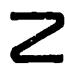
\includegraphics[keepaspectratio]{images/part003_63c67829.jpg}}

推论。设 A 是完全整闭整环，a 是 A 的除性分式理想。则对于 A 的每个非零分式理想 \(\mathfrak{b} \neq 0\)，有 \(\operatorname{div}(\mathfrak{a}: \mathfrak{b}) = \operatorname{div} \mathfrak{a} - \operatorname{div} \mathfrak{b}\)。

由第 1 节的公式 (1)：

\[
\operatorname{div} (a: b) = \operatorname{div} \left(\bigcap_ {\gamma \in b, \gamma \neq 0} \gamma ^ {- 1} a\right) = \sup _ {\gamma \in b, \gamma \neq 0} \operatorname{div} (\gamma ^ {- 1} a)
\]

这里用到了命题 2 以及分式理想 \(y^{-1}\mathfrak{a}\) 是除性的事实。不过，由于 \(\mathrm{D(A)}\) 是有序群（《代数》第 VI 章，§ 1，第 8 节）：

\[
\sup _ {\gamma \in b, \gamma \neq 0} \operatorname{div} (\gamma ^ {- 1} a) = \sup _ {\gamma \in b, \gamma \neq 0} (\operatorname{div} a - \operatorname{div} (\gamma)) = \operatorname{div} a - \inf _ {\gamma \in b, \gamma \neq 0} \operatorname{div} (\gamma) = \operatorname{div} a - \operatorname{div} b.
\]

\subsection{KRULL 整环}

定义 3. 若整环 A 存在一个族

\((v_{\iota})_{\iota\in I}\) 的赋值，它们定义在 A 的分式域 \(\mathbf{K}\) 上并满足以下性质：

(AK \(_{I}\) ) 赋值 \(v_{\iota}\) 是离散的；

(AK \(_{II}\) ) 各个 v \(_{\iota}\) 的赋值环的交为 A；

\((\mathbf{A}\mathbf{K}_{\mathrm{III}})\) 对所有 \(x \in \mathbf{K}^*\)，指标 \(\iota \in \mathbf{I}\) 中满足 \(v_{\iota}(x) \neq 0\) 的集合是有限的。

显然，只需对 A - (0) 中的元素 x 验证条件 \((\mathrm{AK}_{\mathrm{III}})\) 即可。

\textbf{例子}\par

\begin{enumerate}
\def\labelenumi{(\arabic{enumi})}
\item
  每个离散赋值环都是 Krull 整环。
\item
  更一般地，每个主理想整环 A 都是 Krull 整环。事实上，设 \((p_{\iota})_{\iota\in I}\) 是 A 的极端元代表系，令 \(v_{\iota}\) 为由 \(p_{\iota}\) 定义在 A 的分式域上的赋值（第 VI 章，§ 3，第 3 节，例 4）。立即可见，族 \((v_{\iota})_{\iota\in I}\) 满足性质 \((\mathbf{AK}_{\mathbf{I}}), (\mathbf{AK}_{\mathbf{II}})\) 和 \((\mathbf{AK}_{\mathbf{III}})\)。
\item
  设 F 是一个域，\((\mathbf{R}_{i})_{1\leqslant i\leqslant n}\) 是 F 的有限个子环组成的族，且这些子环都是 Krull 整环。则它们的交 \(S=\bigcap_{j=1}^{n}R_{j}\) 是 Krull 整环。对 \(1\leqslant j\leqslant n\)，设 \((v_{j\iota})_{\iota\in I_j}\) 是定义在 \(R_{j}\) 的分式域上、满足 \((\mathrm{AK}_{\mathrm{I}}),(\mathrm{AK}_{\mathrm{II}}),(\mathrm{AK}_{\mathrm{III}})\) 的赋值族（其中以 \(R_{j}\) 代替 A）。记 \(w_{j\iota}\) 为 \(v_{j\iota}\) 在 S 的分式域上的限制。则族 \((v_{j\iota})_{1\leqslant j\leqslant n,\iota\in I_j}\) 显然满足 \((\mathrm{AK}_{\mathrm{II}})\)（其中以 S 代替 A），并且也满足 \((\mathrm{AK}_{\mathrm{III}})\)，因为指标 j 的集合是有限的。赋值 \(w_{j\iota}\) 或者是离散的，或者是不正规的。只保留其中离散的赋值，便得到一个显然满足 \((\mathrm{AK}_{\mathrm{I}}),(\mathrm{AK}_{\mathrm{II}})\) 和 \((\mathrm{AK}_{\mathrm{III}})\) 的族（其中以 S 代替 A）。因此 S 确实是 Krull 整环。
\item
  特别地，如果 A 是 Krull 整环，且 \(K'\) 是 A 的分式域 K 的子域，则 \(K' \cap A\) 是 Krull 整环。
\end{enumerate}

定理 2. 设 A 是整环。A 为 Krull 整环的充要条件是满足以下两个条件：

\begin{enumerate}
\def\labelenumi{(\alph{enumi})}
\item
  A 是完全整闭的；
\item
  \(\mathbf{A}\) 的每个非空除性整理想族都有一个极大元（相对于关系 \(\subset\)）。
\end{enumerate}

此外，若 \(\mathrm{P}(\mathrm{A})\) 是 \(\mathrm{D}(\mathrm{A})\) 的极端元集合，则 \(\mathrm{P}(\mathrm{A})\) 是 Z-模 \(\mathrm{D}(\mathrm{A})\) 的一组基，而 \(\mathrm{D}(\mathrm{A})\) 的正元正是以 \(\mathrm{P}(\mathrm{A})\) 的元素为线性组合、系数满足 \(\geqslant0\) 的那些元素。

设 A 是 Krull 整环。它是完全整闭的（第 VI 章，§ 4，第 5 节，命题 9 的推论）。设 \((v_{\iota})_{\iota\in I}\) 是定义在 A 的分式域 K 上、满足 \((\mathrm{AK}_{\mathrm{I}})\)、\((\mathrm{AK}_{\mathrm{II}})\) 和 \((\mathrm{AK}_{\mathrm{III}})\) 的赋值族。可设 \(v_{\iota}\) 都是赋范的（第 VI 章，§ 3，第 6 节，定义 3）。对于所有 \(\mathfrak{a} \in \mathrm{I}(\mathbf{A})\)，记：

\[
v _ {\iota} (\mathfrak{a}) = \sup _ {\mathfrak{a} \subset Ax} (v _ {\iota} (x));\tag{3}
\]

于是 \(v_{\iota}(\mathfrak{a}) \in \mathbf{Z}\)。事实上，若 \(a\) 是 \(\mathfrak{a}\) 的非零元，关系 \(Ax \supset Aa\) 蕴含 \(v_{\iota}(x) \leqslant v_{\iota}(a)\)（由 \((\mathrm{AK}_{\mathrm{II}})\)），这说明 \(v_{\iota}(x)\)（\(\mathfrak{a} \subset Ax\)）组成的族有上界。我们建立以下性质：

\begin{enumerate}
\def\labelenumi{(\arabic{enumi})}
\tightlist
\item
  设 \(\mathfrak{a}\) 是除性分式理想；\(y \in \mathfrak{a}\) 的充要条件是 \(v_{\iota}(y) \geqslant v_{\iota}(\mathfrak{a})\) 对所有 \(\iota \in \mathbf{I}\) 都成立。
\end{enumerate}

由于 \(\mathfrak{a}\) 是除性的，关系 \(y \in \mathfrak{a}\) 等价于关系“\(\mathfrak{a} \subset \mathbf{A}x\) 蕴含 \(y \in \mathbf{A}x\)”。现在，由 \((\mathrm{AK}_{\mathrm{II}})\)，关系 \(y \in \mathbf{A}x\) 等价于“\(v_{\iota}(y) \geqslant v_{\iota}(x)\) 对所有 \(\iota \in \mathbf{I}\) 都成立”。从而得到 (1)。

\begin{enumerate}
\def\labelenumi{(\arabic{enumi})}
\setcounter{enumi}{1}
\tightlist
\item
  设 \(\mathfrak{a}\) 和 \(\mathfrak{b}\) 是 \(\mathbf{A}\) 的两个除性分式理想；\(\mathfrak{a} \subset \mathfrak{b}\) 的充要条件是 \(v_{\iota}(\mathfrak{a}) \geqslant v_{\iota}(\mathfrak{b})\) 对所有 \(\iota \in \mathbf{I}\) 都成立。
\end{enumerate}

这立即由性质 (1) 得出。

\begin{enumerate}
\def\labelenumi{(\arabic{enumi})}
\setcounter{enumi}{2}
\tightlist
\item
  若 \(x \in \mathbf{K}^*\)，则 \(v_{\iota}(\mathbf{A}x) = v_{\iota}(x)\)。
\end{enumerate}

若 \(A y \supset A x\)，则 \(v_{\iota}(y) \leqslant v_{\iota}(x)\)（由 \((\mathbf{A K}_{\mathrm{II}})\)），且 \(v_{\iota}(y)\) 的最小值在 \(y = x\) 处取得。

\begin{enumerate}
\def\labelenumi{(\arabic{enumi})}
\setcounter{enumi}{3}
\tightlist
\item
  对所有 \(\mathfrak{a} \in \mathbf{I}(\mathbf{A})\)，指标 \(\iota \in \mathbf{I}\) 中满足 \(v_{\iota}(\mathfrak{a}) \neq 0\) 的数目是有限的。
\end{enumerate}

存在 \(x, y\)（属于 \(\mathbf{K}^*\)），使得 \(Ax \subset \mathfrak{a} \subset Ay\)。由性质 (2) 和 (3)，\(v_{\iota}(x) \geqslant v_{\iota}(\mathfrak{a}) \geqslant v_{\iota}(y)\) 对所有 \(\iota \in I\) 都成立。于是只需应用 \((\mathrm{AK}_{\mathrm{III}})\) 即可。

因此我们证明了以下引理：

引理 1. 若 A 是 Krull 整环，且 \((v_{\iota})_{\iota \in I}\) 是定义在 K 上、满足 \((\mathrm{AK}_{\mathrm{I}})\)、\((\mathrm{AK}_{\mathrm{II}})\) 和 \((\mathrm{AK}_{\mathrm{III}})\) 的赋范赋值族，则映射 \(\mathfrak{a} \mapsto (v_{\iota}(\mathfrak{a}))_{\iota \in I}\) 将 A 的除性整理想集合（按 \(\subset\) 排序）递减且单射地映入有序群直和 \(\mathbf{Z}^{(I)}\) 的正元集合。

既然如此，\(\mathbf{Z}^{(I)}\) 的每个非空正元集合都有极小元（《代数》第 VI 章，§ 1，第 13 节，定理 2）。因此 A 确实满足该命题的性质 (b)。

反之，设 A 是满足该命题性质 (a) 和 (b) 的整环。由于 A 完全整闭，D(A) 是有序群（第 2 节，定理 1）。这个群是格（第 1 节，命题 2）。由该命题的条件 (b)，D(A) 的每个非空正元族都有极小元。设 P(A) 是 D(A) 的极端元集合。于是（《代数》第 VI 章，§ 1，第 13 节，定理 2）P(A) 是 Z-模 D(A) 的一组基，而 D(A) 的正元是 P(A) 的元素以正整数为系数的线性组合。
 
因此，对于 \(x \in \mathbf{K}^*\)，可以通过下式定义有理整数 \(v_{\mathbb{P}}(x)\)（其中 \(\mathbf{P} \in \mathbb{P}(\mathbf{A})\)）：

\[
\operatorname{div} (x) = \sum_ {\mathbf {P} \in \mathbf {P} (\mathbf {A})} v _ {\mathbf {P}} (x) \cdot \mathbf {P}.\tag{4}
\]

并记 \(v_{\mathbf{P}}(0) = +\infty\)。

由以下关系

\[
\operatorname{div} (x y) = \operatorname{div} (x) + \operatorname{div} (y)
\]

以及

\[
\operatorname{div} (x + y) \geqslant \inf (\operatorname{div} (x), \operatorname{div} (y)),
\]

对于 \(x, y\) 及 \(x + y\)（均属于 \(\mathbf{K}^*\)），我们推出 \(v_{\mathbb{P}}\) 是 \(\mathbf{K}\) 上的离散赋值。\(x \in \mathbf{A}\) 的充要条件是 \(\mathrm{div}(x) \geqslant 0\)，也就是 \(v_{\mathbb{P}}(x) \geqslant 0\) 对所有 \(\mathbb{P} \in \mathbb{P}(\mathbf{A})\) 都成立。因此，\(v_{\mathbb{P}}\) 满足条件 \((\mathbf{AK}_{\mathbf{I}})\) 和 \((\mathbf{AK}_{\mathbf{II}})\)，显然也满足 \((\mathbf{AK}_{\mathbf{III}})\)。

推论。诺特环为 Krull 整环的充要条件是它是整闭整环。

整闭的诺特整环是完全整闭的（第 V 章，§ 1，第 4 节）。

存在非诺特的 Krull 整环，例如域 K 上、具有无穷多个不定元的多项式环 \(K[X_{n}]_{n\in\mathbf{N}}\)（参见习题 8）。

\subsection{KRULL 整环的本性赋值}

设 A 是 Krull 整环，K 是其分式域。第 3 节的公式 (4) 定义的赋值（对 \(x \in \mathbf{K}^*\)）称为 K（或 A）的本性赋值。

我们在定理 2 的证明过程中已经指出，赋值 \(v_{\mathbb{P}}\) 满足定义 3 的性质 \((\mathrm{AK}_{\mathbb{I}}), (\mathrm{AK}_{\mathbb{II}})\) 和 \((\mathrm{AK}_{\mathbb{III}})\)。此外，这些离散赋值 \(v_{\mathbb{P}}\) 是赋范的：对于每个极端除子 \(\mathbf{P} \in \mathbf{P}(\mathbf{A})\)，有 \(\mathbf{P} < 2\mathbf{P}\)，因而若 \(\mathfrak{a}\) 和 \(\mathfrak{b}\) 是分别对应于 \(\mathbf{P}\) 和 \(2\mathbf{P}\) 的除性理想，则 \(\mathfrak{a} \supset \mathfrak{b}\) 且 \(\mathfrak{a} \neq \mathfrak{b}\)；对于 \(x \in \mathfrak{a} - \mathfrak{b}\)，有 \(\operatorname{div}(x) \geqslant \mathbf{P}\) 且 \(\operatorname{div}(x) \not\geqslant 2\mathbf{P}\)，从而 \(v_{\mathbb{P}}(x) = 1\)，这就证明了断言。

命题 5. 设 A 是 Krull 整环，K 是其分式域，\((v_{\mathbf{P}})_{\mathbf{P} \in \mathbf{P}(\mathbf{A})}\) 是其本性赋值族。设 \((n_{\mathbf{P}})_{\mathbf{P} \in \mathbf{P}(\mathbf{A})}\) 是一个有理整数族，除有限个指标外其余值均为零。则集合 \(x \in \mathbf{K}\)，满足 \(v_{\mathbf{P}}(x) \geqslant n_{\mathbf{P}}\) 对所有 \(\mathbf{P} \in \mathbf{P}(\mathbf{A})\) 都成立，正是除性理想 \(\mathfrak{a}\)（\(\mathbf{A}\) 的），且 \(\operatorname{div} \mathfrak{a} = \sum_{\mathbf{P} \in \mathbf{P}(\mathbf{A})} n_{\mathbf{P}} \cdot \mathbf{P}\)。

令 \(x \in K^*\)。\(x \in a\) 的充要条件是 \(Ax \subset a\)，从而等价于 \(\operatorname{div}(x) \geqslant \operatorname{div} a\)，进而由 (4) 等价于 \(v_{\mathbf{P}}(x) \geqslant n_{\mathbf{P}}\) 对所有 \(\mathbf{P} \in \mathbf{P}(\mathbf{A})\) 都成立。

命题 6. 设 A 是 Krull 整环，K 是其分式域，\((v_{\iota})_{\iota \in I}\) 是 K 上满足定义 3 中性质的赋值族，\(\mathbf{A}_{\iota}\) 是 \(v_{\iota}\) 的赋值环。设 S 是 A 的不含 0 的乘性子集，J 是指标 \(\iota \in I\) 中满足 \(v_{\iota}\) 在 S 上为零者的集合。则 \(\mathrm{S}^{-1}\mathrm{A} = \bigcap_{\iota \in I}\mathrm{A}_{\iota}\)；特别地，\(\mathrm{S}^{-1}\mathrm{A}\) 是 Krull 整环。

记 \(\mathbf{B} = \bigcap_{\iota \in \mathbf{J}} \mathbf{A}_{\iota}\)。则 \(\mathbf{S}^{-1} \subset \mathbf{B}\) 且 \(\mathbf{A} \subset \mathbf{B}\)，从而 \(\mathbf{S}^{-1}\mathbf{A} \subset \mathbf{B}\)。反之，设 \(x \in \mathbf{B}\)。记 \(\mathbf{J}'\) 为指标 \(\iota\) 中满足 \(v_{\iota}(x) < 0\) 的有限集合。若 \(\iota \in \mathbf{J}'\)，则 \(x \notin \mathbf{A}_{\iota}\)，从而 \(\iota \notin \mathbf{J}\)，因而存在 \(s_{\iota} \in \mathbf{S}\) 使 \(v_{\iota}(s_{\iota}) > 0\)。取 \(n(\iota)\) 为一个整数 \(>0\)，使得 \(v_{\iota}(s_{\iota}^{n(\iota)}x) \geqslant 0\)；记 \(s = \prod_{\iota \in \mathbf{J}} s_{\iota}^{n(\iota)}\)。于是 \(v_{\iota}(sx) \geqslant 0\) 对所有 \(\iota \in \mathbf{I}\) 都成立，从而 \(sx \in \mathbf{A}\) 且 \(x \in \mathbf{S}^{-1}\mathbf{A}\)。因此 \(\mathbf{B} = \mathbf{S}^{-1}\mathbf{A}\)。

推论 1. 设 P 是 A 的一个极端除子，p 是相应的除性理想。则 p 是素理想，\(v_{\mathbf{P}}\) 的赋值环是 \(A_{\mathfrak{p}}\)，且 \(v_{\mathbf{P}}\) 的剩余域可与 A/p 的分式域相识别。

令 \(S = A - p\)。由命题 5，\(v_{P}\) 在 \(S\) 上为零，且 \(>0\) 在 \(p\) 上成立。因此，\(p\) 是 \(A\) 与 \(v_{P}\) 的理想的交，因而是素理想。另一方面，对于每个极端除子 \(Q \neq P\)，都有 \(Q \not\geq P\)，所以除性理想 \(q\)（对应于 \(Q\)）不包含于 \(p\)；于是 \(q \cap S \neq \varnothing\)，从而由命题 5，\(v_{Q}\) 在 \(S\) 上不为零。由此，推论由命题 6 及第 II 章，§ 3，第 1 节，命题 3 得出。

推论 2. 设 A 是 Krull 整环，K 是其分式域，\((v_{\iota})_{\iota\in I}\) 是满足定义 3 中性质的赋值族。则 A 的每个本性赋值都等价于某个 \(v_{\iota}\)。

设 P 是 A 的一个极端除子，p 是相应的除性理想。由推论 1、命题 5、引理 1 以及第 3 节定理 2 的证明中的断言 (1)，存在 \(\iota \in I\)，使得赋值环 \(A_{\iota}\)（属于 \(v_{\iota}\)）包含赋值环 \(A_{p}\)（属于 \(v_{P}\)）。由于 \(v_{\iota}\) 和 \(v_{P}\) 的高度都是 1，它们因而等价（第 VI 章，§4，第 5 节，命题 6）。

命题 7. 设 A 是 Krull 整环，\((v_{\mathbb{P}})_{\mathbb{P} \in \mathbb{P}(\mathbb{A})}\) 是其本性赋值族，且 \(\mathfrak{a} \in \mathbf{I}(\mathbf{A})\)。则 div \(\mathfrak{a}\) 中 P 的系数是 \(\inf_{y \in \mathfrak{a}} (v_{\mathbb{P}}(y))\)。若 \(\mathfrak{p}\) 是对应于极端除子 P 的除性素理想，则 \(\mathfrak{a}\mathrm{A}_{\mathfrak{p}} = \tilde{\mathfrak{a}}\mathrm{A}_{\mathfrak{p}}\)。

由于 \(\mathfrak{a} = \sum_{y \in \mathfrak{a}} Ay\)，第 1 节的命题 2 (b) 表明 \(\text{div}(\mathfrak{a}) = \inf_{y \in \mathfrak{a}} (\text{div}(Ay))\)，从而得到第一个断言。第二个断言立即成立，因为 \(\text{div} \tilde{\mathfrak{a}} = \text{div} \mathfrak{a}\)，且 \(A_{\mathfrak{p}}\) 是离散赋值 \(v_{\mathfrak{p}}\) 的赋值环。

命题 8. 设 A 是整闭的诺特整环。

\begin{enumerate}
\def\labelenumi{(\alph{enumi})}
\tightlist
\item
  设 \(\mathbf{P}\) 是 \(\mathbf{A}\) 的一个极值除子，\(\mathfrak{p}\) 是相应的除性素理想；
\end{enumerate}

对于 \(n \in \mathbf{N}\)，令 \(\mathfrak{p}^{(n)} = \mathfrak{p}^n\mathbf{A}_{\mathfrak{p}} \cap \mathbf{A}\)；则 \(\mathfrak{p}^{(n)}\) 是 \(x \in \mathbf{A}\) 的集合，其中 \(v_{\mathfrak{p}}(x) \geqslant n\)，并且是一个 \(\mathfrak{p}\)-准素理想。

\begin{enumerate}
\def\labelenumi{(\alph{enumi})}
\setcounter{enumi}{1}
\tightlist
\item
  设 \(\mathfrak{a}\) 是除性整理想，\(n_1\mathrm{P}_1 + \dots + n_r\mathrm{P}_r\) 是 \(\mathfrak{a}\) 的除子（其中 \(\mathbf{P}_i\) 是互异的极端除子），\(\mathfrak{p}_i\) 是对应于 \(\mathbf{P}_i\) 的除性素理想。
\end{enumerate}

则 \(\mathfrak{a} = \bigcap_{i=1}^{r} \mathfrak{p}_i^{(n_i)}\) 是 \(\mathfrak{a}\) 的唯一既约准素分解，且 \(\mathfrak{p}_i\) 不是浸入的。

由命题 6 的推论 1，关系 \(x \in \mathfrak{p}^n\mathrm{A}_{\mathfrak{p}} = (\mathfrak{p}\mathrm{A}_{\mathfrak{p}})^n\) 等价于 \(v_{\mathfrak{p}}(x) \geqslant n\)；另一方面，由于 \(\mathrm{A}_{\mathfrak{p}}\) 是离散赋值环，\((\mathfrak{p}\mathrm{A}_{\mathfrak{p}})^n\) 是 \((\mathfrak{p}\mathrm{A}_{\mathfrak{p}})\)-准素理想（第 IV 章，§ 2，第 1 节，例 4），从而 \(\mathfrak{p}^{(n)}\) 是 \(\mathfrak{p}\)-准素理想（第 IV 章，§ 2，第 1 节，命题 3）；这就证明了 (a)。命题 5 显然证明了 \(\mathfrak{a} = \bigcap_{i=1}^{r} \mathfrak{p}_i^{(n_i)}\)。由于 \(\mathfrak{p}_i \not\subset \mathfrak{p}_j\) 对 \(i \neq j\) 成立，这个准素分解是既约的：事实上，若 \(\mathfrak{p}_i^{(n_i)} \supset \bigcap_{j \neq i} \mathfrak{p}_j^{(n_j)} \supset \prod_{j \neq i} \mathfrak{p}_j^{(n_j)}, \mathfrak{p}_i\) 将包含某个 \(\mathfrak{p}_j\)，其中 \(j \neq i\)（第 II 章，§ 1，第 1 节，命题 1）。唯一性由第 IV 章，§ 2，第 3 节，命题 5 得出。

\subsection{本性赋值的逼近}

由于 Krull 整环的本性赋值是离散且赋范的，任意两个本性赋值都不等价，因而它们是独立的（第 VI 章，§ 7，第 2 节）。因此可以对它们应用逼近定理的推论 2（同上，定理 1）：给定一些 \(n_i \in \mathbf{Z}\) 以及有限个互异的本性赋值 \(v_i\)，存在 \(x \in \mathbf{K}\)，使得 \(v_i(x) = n_i\) 对所有 \(i\) 都成立。不过，这里有一个更精确的结果：

命题 9. 设 \(v_1, \ldots, v_r\) 是 Krull 整环 A 的互异本性赋值，\(n_1, \ldots, n_r\) 是有理整数。则 A 的分式域 K 中存在元素 \(x\)，使得 \(v_i(x) = n_i\) 对 \(1 \leqslant i \leqslant r\) 都成立，并且 \(v(x) \geqslant 0\) 对 A 的每个本性赋值 \(v\)（不同于 \(v_1, \ldots, v_r\)）都成立。

设 \(\mathfrak{p}_1, \ldots, \mathfrak{p}_r\) 是分别对应于赋值 \(v_1, \ldots, v_r\) 的 A 的除性理想。存在 \(y \in K\)，使得 \(v_i(y) = n_i\) 对 \(1 \leqslant i \leqslant r\) 都成立（第 VI 章，§ 7，第 2 节，定理 1 的推论 1）。A 的本性赋值 \(w_1, \ldots, w_s\) 不同于 \(v_i\)，且 \(w_j(y) = -m_j\) 满足 \(<0\)，其数目是有限的；设相应的理想为 \(\mathfrak{q}_1, \ldots, \mathfrak{q}_s\)。\(\mathfrak{p}_1, \ldots, \mathfrak{p}_r, \mathfrak{q}_1, \ldots, \mathfrak{q}_s\) 之间不存在包含关系，因为这些理想对应于极端除子，而这些理想是素理想（命题 6 的推论 1）。因此，整理想 \(\mathfrak{a} = \mathfrak{q}_1^{m_1} \ldots \mathfrak{q}_s^{m_s}\) 不包含于任何一个 \(\mathfrak{p}_i\)（第 II 章，§ 1，第 1 节，命题 1），所以也不包含于它们的并中（同上，命题 2）。因此存在 \(z \in \mathfrak{a}\)，使得 \(z \notin \mathfrak{p}_i\) 对 \(1 \leqslant i \leqslant r\) 都成立；于是 \(v_1(z) = \cdots = v_r(z) = 0\)，且 \(w_j(z) \geqslant m_j\) 对 \(1 \leqslant j \leqslant s\) 都成立；从而元素 \(x = yz\) 解决了问题。

推论 1. 设 A 是 Krull 整环，K 是其分式域，a、b、c 是 A 的三个除性分式理想，且 a ⊂ b。则存在 x ∈ K，使得 a = b ∩ xc。

设 \((v_{\iota})_{\iota \in I}\) 是 A 的本性赋值族，设 \((m_{\iota})\)（分别地，\((n_{\iota})\)、\((p_{\iota})\)）是一个有理整数族（除有限个指标外其余值均为零），使得 \(\mathfrak{a}\)（分别地，\(\mathfrak{b}, \mathfrak{c}\)）是 \(x \in K\) 的集合，其中 \(v_{\iota}(x) \geqslant m_{\iota}\)（分别地，\(n_{\iota}, p_{\iota}\)）对所有 \(\iota \in I\) 都成立（命题 5，第 4 节）。集合 J 由指标 \(\iota \in I\) 中满足 \(m_{\iota} > n_{\iota}\) 的组成，且 J 是有限的。由于除有限个指标外 \(p_{\iota} = m_{\iota} = 0\)，命题 9 表明存在 \(x \in K^{*}\)，使得 \(v_{\iota}(x^{-1}) + m_{\iota} = p_{\iota}\) 对 \(\iota \in J\) 成立，并且

\[
v _ {\iota} (x ^ {- 1}) + m _ {\iota} \geqslant p _ {\iota}
\]

当 \(\iota \in \mathbf{I} - \mathbf{J}\) 时成立。于是对所有 \(\iota \in \mathbf{I}\)，\(m_{\iota} = \sup (n_{\iota}, v_{\iota}(x) + p_{\iota})\)。从而 \(\mathfrak{a} = \mathfrak{b} \cap x\mathfrak{c}\)。

推论 2. 设 A 是 Krull 整环。A 的分式理想 \(\mathfrak{a}\) 为除性的充要条件是它是两个分式主理想的交。

充分性显然（第 1 节，定义 2）。必要性由推论 1 得出：取 b 和 c 为主理想，并使 b ⊃ a。

\subsection{KRULL 整环中的高度 1 素理想}

定义 4. 设 A 是整环。若 A 的素理想 p 在 A 的非零素理想中是极小的，就称 p 的高度为 1。

我们也称理想 (0) 的高度为 0；因此，按定义，高度 \(\leqslant 1\) 的素理想等于 (0) 或者高度为 1。

下面我们将以一般方式定义素理想的高度。

定理 3. 设 A 是 Krull 整环，p 是 A 的整理想。p 是对应于某个极端除子的除性理想的充要条件是 p 是高度为 1 的素理想。

若 p 是对应于某个极端除子的除性理想，我们知道（第 4 节，命题 6 的推论 1）p 是素理想且 \(A_{p}\) 是离散赋值环；由于 \(A_{p}\) 除了 (0) 和 \(pA_{p}\) 外没有其他素理想，(0) 和 p 就是包含于 p 的 A 的唯一素理想（第 II 章，§ 3，第 1 节，命题 3）；因此 p 的高度为 1。反之，我们先证明每个 \(p \neq (0)\) 的 A 的素理想都包含一个对应于极端除子的除性素理想 q：因为 \(A_{p} \neq K\)，所以 \(A_{p}\) 是非空族（\(A_{t}\)）的本性赋值环的交（第 4 节，命题 6）；每个 \(A_{t}\) 都具有 \(A_{q_{t}}\) 的形式（第 4 节，命题 6 的推论 1），由 \(A_{p} \subset A_{q_{t}}\) 可推出 \(q_{t} \subset p\)。因此，若 p 的高度为 1，则 p = q，这说明 p 是对应于某个极端除子的除性理想。

推论 1. 在 Krull 整环中，每个非零素理想 m 都包含一个高度为 1 的素理想。若 m 的高度不是 1，则 div m = 0 且 A: m = A。

第一个断言已经在定理 3 的证明过程中得到。若 \(m\) 的高度不是 1，且 \(p\) 是一个高度为 1 的素理想并包含于 \(m\)，则 \(p \subset \tilde{m}\) 且 \(p \neq \tilde{m}\)；由于 \(\text{div } p\) 是极端的，必有 \(\text{div } m = \text{div } \tilde{m} = 0\)；从而 \(\text{div}(A: m) = 0\)，又因为 \(A: m\) 是除性的（第 1 节，命题 1），所以 \(A: m = A\)。

推论 2. 设 A 是 Krull 整环，K 是其分式域，v 是 K 上在 A 上为正的赋值，p 是 \(x \in A\) 中满足 \(v(x) > 0\) 的元素的集合。若素理想 p 的高度为 1，则 v 等价于 A 的一个本性赋值。

设 \(B\) 是 \(v\) 的赋值环，\(m\) 是其理想。则 \(m \cap A = p\)，从而 \(A_p \subset B\)。现在 \(A_p\) 是离散赋值环（定理 3 以及命题 6 的推论 1）。由于 \(p \neq (0)\)，\(B \neq K\)，因而 \(B = A_p\)（第 VI 章，§ 4，第 5 节，命题 6）。

定理 4. 设 A 是整环，M 是其高度为 1 的素理想集合。A 为 Krull 整环的充要条件是满足以下性质：

\begin{enumerate}
\def\labelenumi{(\roman{enumi})}
\item
  对所有 \(\mathfrak{p} \in \mathbf{M}\)，\(\mathbf{A}_{\mathfrak{p}}\) 都是离散赋值环。
\item
  A 是各个 \(\mathbf{A}_{\mathfrak{p}}\) 的交，其中 \(\mathfrak{p} \in \mathbf{M}\)。
\item
  对所有 \(x \neq 0\)（属于 \(\mathbf{A}\)），指标 \(\mathfrak{p} \in \mathbf{M}\) 中满足 \(x \in \mathfrak{p}\) 的至多有有限个。
\end{enumerate}

此外，与 \(A_{p}\) 对应的、其中 \(p \in M\) 的赋值正是 A 的本性赋值。

这些条件显然充分。其必要性立即由第 4 节的定理 3、命题 6 的推论 1 以及 A 的本性赋值满足第 3 节定义 3 的条件这一事实得出。

命题 10. 设 A 是整闭的诺特整环，a 是 A 的整理想。以下条件等价：

\begin{enumerate}
\def\labelenumi{(\alph{enumi})}
\item
  a 是除性的；
\item
  与 A/a 相伴的素理想都具有高度1。
\end{enumerate}

回忆一下，若 \(a = \bigcap_{i=1}^{n} q_i\) 是 a 的既约准素分解，且 \(p_i\) 表示对应于 \(q_i\) 的素理想，则与 A/a 相伴的素理想正是 \(p_i\)（第 IV 章，§2，第 3 节，命题 4）。于是 (a) 蕴含 (b) 由第 4 节的命题 8 得出。反之，若在上述记号下 \(p_i\) 的高度为 1，则 \(A_{p_i}\) 是离散赋值环（定理 4）；现在，\(q_i = q_i A_{p_i} \cap A\)（第 IV 章，§2，第 1 节，命题 3）；记 \(v_i\) 为对应于 \(p_i\) 的本性赋值，则存在整数 \(n_i\)，使得 \(q_i\) 是 \(x \in A\) 的集合，其中 \(v_i(x) \geqslant n_i\)；这说明 \(q_i\) 是除性的（第 4 节，命题 5），从而 a 也是除性的。

\subsection{应用：离散赋值环的新刻画}

命题 11. 设 A 是局部 Krull 整环（特别地，是整闭的局部诺特整环），m 是其极大理想。以下条件等价：

\begin{enumerate}
\def\labelenumi{(\alph{enumi})}
\item
  A 是离散赋值环；
\item
  m 是可逆的；
\item
  A: m ≠ A；
\item
  m 是除性的；
\item
  m 是 A 的唯一非零素理想。
\end{enumerate}

由于离散赋值环的每个非零理想都是主理想（第 VI 章，§ 3，第 6 节，命题 9），它是可逆的，从而 (a) 蕴含 (b)。若 m 可逆，其逆是 A: m（第 II 章，§ 5，第 6 节，命题 10），因此 A: m ≠ A；从而 (b) 蕴含 (c)。若 A: m ≠ A，则 A: (A: m) ≠ A；现在 m ⊂ A: (A: m)；由于 m 是极大理想，故 m = A: (A: m)，所以 m 是除性的（第 1 节，命题 1 (c)）；从而 (c) 蕴含 (d)。(d) 蕴含 (e) 由第 6 节的定理 3 得出。最后，若 m 是 A 的唯一非零素理想，则其高度为 1，因而 A \(_{m}\) 是离散赋值环（第 6 节，定理 4）；由于 A 是局部环，A \(_{m}\) = A，这说明 (e) 蕴含 (a)。

\subsection{Krull 整环在其分式域有限扩张中的整闭包}

命题 12. 设 A 是 Krull 整环，K 是其分式域，K' 是 K 的有限扩张，A' 是 A 在 K' 中的整闭包。则 A' 是 Krull 整环。A' 的本性赋值是 K' 上与 A 的本性赋值的扩张等价的赋范离散赋值。

设扩张族 \((v_{\iota})_{\iota\in I}\)（扩张到 \(K'\)）由 A 的本性赋值得到。由于次数 \(n = [K':K]\) 有限，赋值 \(v_{\iota}\) 是 \(K'\) 上的离散赋值（第 VI 章，§ 8，第 1 节，命题 1 的推论 3）。令 \(B_{\iota}\) 为 \(v_{\iota}\) 的赋值环；则 \(A' \subset \bigcap_{\iota\in I}B_{\iota}\)（第 VI 章，§ 1，第 3 节，定理 3）。反之，每个元素 \(x\)（属于 \(\bigcap_{\iota\in I}B_{\iota}\)）都整依赖于 A 的每个本性赋值环（第 VI 章，§ 1，第 3 节，定理 3 的推论 3）；因此 \(x\) 在 K 上的极小多项式的系数属于 A（第 V 章，§ 1，第 3 节，命题 11 的推论），所以 \(x\in A'\)；从而 \(A' = \bigcap_{\iota\in I}B_{\iota}\)。现在令 \(x\) 为 \(A'\) 的非零元素；它满足形如 \(x^{s} + a_{s-1}x^{s-1} + \cdots + a_{0} = 0\) 的方程，其中 \(a_{i}\in A\) 且 \(a_{0}\neq 0\)；若 \(v_{\iota}(x) > 0\)，则 \(v_{\iota}(a_{0}) > 0\)；现在，A 的本性赋值 \(v\) 中满足 \(v(a_{0}) > 0\) 的只有有限个，而 \(K'\) 上延拓 K 上给定赋值的赋值也只有有限个（第 VI 章，§ 8，第 3 节，定理 1）；因而 \(v_{\iota}(x) = 0\)，除了有限个指标 \(\iota\in I\) 外。这样便证明了 \(A'\) 是 Krull 整环（第 3 节，定义 3）。

还需证明 \(v_{\iota}\) 与 \(A'\) 的本性赋值等价（第 4 节，命题 6 的推论 2），也就是（第 6 节，定理 3 的推论 2）证明素理想 \(\mathfrak{p}_{\iota}\)（由 \(x \in A'\) 中满足 \(v_{\iota}(x) > 0\) 的元素组成）具有高度 1。若非如此，则存在素理想 \(\mathfrak{q}\)，它是 \(A'\) 的素理想，并满足 \((0) \subset \mathfrak{q} \subset \mathfrak{p}_{\iota}\)，且不同于 (0) 和 \(\mathfrak{p}_{\iota}\)；于是 \((0) \subset \mathfrak{q} \cap A \subset \mathfrak{p}_{\iota} \cap A\)，并且 \(\mathfrak{q} \cap A\) 不同于 (0) 和 \(\mathfrak{p}_{\iota} \cap A\)（第 V 章，§ 2，第 1 节，命题 1 的推论 1）；因此素理想 \(\mathfrak{p}_{\iota} \cap A\) 的高度不为 1，这与它对应于 \(A\) 的本性赋值这一事实矛盾。

推论。设 \(\mathfrak{p}\)（分别地，\(\mathfrak{p}'\)）是 A（分别地，A'）的高度为 1 的素理想，\(v\)（分别地，\(v'\)）是与之对应的 A（分别地，A'）的本性赋值。\(\mathfrak{p}'\) 位于 \(\mathfrak{p}\) 之上的充要条件是 \(v'\) 在 K 上的限制等价于 \(v\)。

赋值 \(v'\) 等价于 A 的本性赋值 w 的扩张（命题 12）。令 \(q = p' \cap A\)，它是 A 的高度为 1 的素理想。\(v'\) 在 K 上的限制等价于 v 的充要条件是 w = v，从而 q = p。

\subsection{Krull 整环上的多项式环}

命题 13. 设 A 是 Krull 整环，\(\mathbf{X}_1, \mathbf{X}_2, \ldots, \mathbf{X}_n\) 是不定元。环 \(\mathrm{A}[\mathbf{X}_1, \ldots, \mathbf{X}_n]\) 是 Krull 整环。

对 n 作归纳，只需证明：若 X 是不定元，则 A{[}X{]} 是 Krull 整环。令 K 为 A 的分式域。A{[}X{]} 的分式域是 K(X)。令 I 为 K{[}X{]} 中在 K 上不可约的首一多项式集合；对于所有 \(f \in I\)，令 \(v_{f}\) 为 K(X) 上由 f 定义的赋值（第 VI 章，§3，第 3 节，例 4）。另一方面，对于 A 的每个本性赋值 w，令 \(\bar{w}\) 为 w 到 K(X) 的扩张，它定义为

\[
\bar {w} \left(\sum_ {j} a _ {j} X ^ {j}\right) = \inf _ {j} (w (a _ {j}))
\]

对于 \(\sum_{j} a_j X^j \in K[X]\)（第 VI 章，§ 10，第 1 节，引理 1）。显然 \(v_f\) 和 \(\bar{w}\) 都是离散且赋范的；对于所有 \(u \in K[X]\)，\(v_f(u) = 0\)（分别地，\(\bar{w}(u) = 0\)）的赋值 \(v_f\)（分别地，\(\bar{w}\)）除有限个外均如此。

为证明命题，只需证明 A{[}X{]} 是赋值 \(v_{f}\) 和 \(\bar{w}\) 的赋值环的交。现在，赋值 \(v_{f}\) 的赋值环的交是 K{[}X{]}。另一方面，对于 \(\sum_{j} a_{j} X^{j} \in K[X]\)，关系 \(\bar{w}\left(\sum_{j} a_{j} X^{j}\right) \geqslant 0\) 等价于“\(w(a_{j}) \geqslant 0\) 对所有 j 都成立”；因此，关系“\(\bar{w}\left(\sum_{j} a_{j} X^{j}\right) \geqslant 0\) 对每个赋值 \(\bar{w}\) 都成立”等价于“\(w(a_{j}) \geqslant 0\) 对所有 j 以及 A 的每个本性赋值 w 都成立”。这就证明了断言。

注。命题 13 的证明中引入的赋值 \(v_f\) 和 \(\bar{w}\) 是 A{[}X{]} 的本性赋值。我们只需证明：若 V 是由赋值 \(v_f\)（\(f\) 不可约）和 \(\bar{w}\)（\(w\) 是本性的）组成的集合，则对每个 \(v' \in V\)，存在元素 \(g \in K(X)\)，它不属于 A{[}X{]}，并且 \(v''(g) \geqslant 0\) 对所有赋值 \(v'' \in V\)（不同于 \(v'\)）都成立；这将证明 \(V - \{v'\}\) 不满足 (AK \(_{\text{II}}\) )，因而结论由第 4 节、命题 6 的推论 2 得出。先假设 \(v'\) 具有 \(\bar{w}\) 的形式：于是可以取 \(g\) 为元素 \(b \in K\)，使得 \(w(b) < 0\)，并且 \(w'(b) \geqslant 0\) 对 A 的本性赋值 \(w'\)（不同于 \(w\)）都成立，因为 \(v_f(b) = 0\) 对每个不可约首一多项式 \(f\)（属于 K{[}X{]}）都成立；满足上述条件的元素 \(b\) 的存在性由第 5 节、命题 9 得出。再假设 \(v'\) 具有 \(v_f\) 的形式，其中 \(f \in K[X]\) 是次数为 \(m\) 的不可约首一多项式；于是可以取 \(g = a/f\)，其中 \(a \in A\)。有 \(v_h(g) \geqslant 0\)（对于每个不可约首一多项式 \(h \neq f\)，它属于 K{[}X{]}）；还需选择 \(a \in A\)，使得对于 A 的每个本性赋值 \(w\)，\(w(a)\) 至少等于元素 \(w(c_i)\) 的最大下界，其中 \(c_i\) 是 \(f (1 \leqslant i \leqslant m)\) 的系数；现在，这样的 \(a \in A\) 的存在性由 (AK \(_{\text{III}}\) ) 及第 5 节、命题 9 得出。

我们还可以说（第 6 节，定理 4），A{[}X{]} 的高度为 1 的素理想是：

\begin{enumerate}
\def\labelenumi{(\arabic{enumi})}
\item
  形如 \(\mathfrak{p}\mathbf{A}[\mathbf{X}]\) 的素理想，其中 \(\mathfrak{p}\) 是 \(\mathbf{A}\) 的高度为 1 的素理想；
\item
  形如 \(\mathfrak{m} \cap \mathrm{A}[\mathrm{X}]\) 的素理想，其中 \(\mathfrak{m}\) 是 \(\mathrm{K}[\mathrm{X}]\) 的（必为主理想的）素理想。
\end{enumerate}

后者的特征是它们与 A 的交化为 0。

\subsection{KRULL 整环的除子类}

设 A 为 Krull 整环。回忆，A 的除子群 D(A) 是由其极值元集合 P(A) 生成的自由交换群（第3节，定理2），且 P(A) 可与 A 的高度为1的素理想集合等同（第6节）；对于 \(p \in P(A)\)，我们把对应于 p 的赋范本性赋值记为 \(v_{p}\)（第4节）；回忆，\(v_{p}\) 的赋值环是 \(A_{p}\)（第4节，命题6后的推论1）。我们把由主除子组成的 D(A) 子群记为 F(A)，把 C(A) = D(A)/F(A) 记为 A 的除子类群（第2节）。

命题14. 设 A 为 Krull 整环，B 为包含 A 的 Krull 整环。假设满足以下条件：

（PDE）对于每个高度为1的素理想 \(\mathfrak{P}\)（属于 \(\mathbf{B}\)），素理想 \(\mathfrak{P} \cap \mathbf{A}\) 为零或具有高度1。

对于 \(\mathfrak{p} \in \mathrm{P}(\mathbf{A})\)，\(\mathfrak{P} \in \mathrm{P}(\mathbf{B})\) 中满足 \(\mathfrak{P} \cap \mathbf{A} = \mathfrak{p}\) 的理想数目有限；记作

\[
i (\mathfrak {p}) = \sum_ {\mathfrak {P} \in \mathrm{P} (\mathrm{B}), \mathfrak {P} \cap \mathrm{A} = \mathfrak {p}} e (\mathfrak {P} / \mathfrak {p}) \mathfrak {P},
\]

其中 \(e(\mathfrak{P} / \mathfrak{p})\) 表示 \(v_{\mathfrak{P}}\) 关于 \(v_{\mathfrak{p}}\) 的分歧指数（第VI章，第8节，第1号）。于是，\(i\) 通过线性性定义了从 D(A) 到 D(B) 的保序同态，并具有以下性质：

\begin{enumerate}
\def\labelenumi{(\alph{enumi})}
\tightlist
\item
  对于每个非零元素 \(x\)（属于 \(\mathbf{A}\) 的分式域），
\end{enumerate}

\[
i \left(\operatorname{div} _ {\mathbf {A}} (x)\right) = \operatorname{div} _ {\mathbf {B}} (x);
\]

\begin{enumerate}
\def\labelenumi{(\alph{enumi})}
\setcounter{enumi}{1}
\tightlist
\item
  对于 D(A) 中的所有 D、D'，
\end{enumerate}

\[
i \left(\sup (\mathbf {D}, \mathbf {D} ^ {\prime})\right) = \sup (i (\mathbf {D}), i (\mathbf {D} ^ {\prime})).
\]

设 \(\mathfrak{p} \in \mathrm{P}(\mathbf{A})\)；取一个非零元素 \(a\)，它属于 \(\mathfrak{p}\)；\(\mathfrak{P} \in \mathrm{P}(\mathbf{B})\) 中包含 \(a\) 的理想数目有限（第6节，定理4）；从而，\(\mathfrak{P} \in \mathrm{P}(\mathbf{B})\) 中满足 \(\mathfrak{P} \cap \mathbf{A} = \mathfrak{p}\) 的理想数目也有限。

现在证明 (a)。由可加性，不妨设 \(x \in \mathbf{A}^* = \mathbf{A} - \{0\}\)。按定义，\(\operatorname{div}_{\mathbf{B}}(x) = \sum_{\mathfrak{P} \in \mathrm{P}(\mathbf{B})} v_{\mathfrak{P}}(x) \cdot \mathfrak{P}\)。对于所有 \(\mathfrak{P} \in \mathrm{P}(\mathbf{B})\)，若 \(v_{\mathfrak{P}}(x) > 0\)，则 \(\mathfrak{P} \cap \mathbf{A}\) 非零（因为 \(x \in \mathfrak{P}\)），由（PDE）可知其具有高度1；令 \(\mathfrak{p} = \mathfrak{P} \cap \mathbf{A}\)，根据分歧指数的定义，\(v_{\mathfrak{P}}(x) = e(\mathfrak{P}/\mathfrak{p})v_{\mathfrak{p}}(x)\)（因为 \(v_{\mathfrak{p}}\) 和 \(v_{\mathfrak{P}}\) 都是赋范的）。又由于 \(\operatorname{div}_{\mathbf{A}}(x) = \sum_{\mathfrak{p} \in \mathrm{P}(\mathbf{A})} v_{\mathfrak{p}}(x) \cdot \mathfrak{p}\)，对于所有满足 \(i(\mathfrak{q}) = 0\) 的 \(\mathfrak{q} \in \mathrm{P}(\mathbf{A})\)，若它不是形如 \(\mathfrak{Q} \cap \mathbf{A}\)（其中 \(\mathfrak{Q} \in \mathrm{P}(\mathbf{B})\)）的理想，即得 (a)。

为证明 (b)，记

\[
\mathrm{D} = \sum_ {\mathfrak {p} \in \mathrm{P} (\mathrm{A})} n (\mathfrak {p}) \cdot \mathfrak {p} \quad \text { and } \quad \mathrm{D} ^ {\prime} = \sum_ {\mathfrak {p} \in \mathrm{P} (\mathrm{A})} n ^ {\prime} (\mathfrak {p}) \cdot \mathfrak {p};
\]

\(\mathfrak{p}\) 在 \(\sup (\mathrm{D},\mathrm{D}^{\prime})\) 中的系数为 \(\sup (n(\mathfrak{p}),n^{\prime}(\mathfrak{p}))\)。设 \(\mathfrak{P}\) 是 \(\mathrm{P(B)}\) 中的元素。若 \(\mathfrak{P}\cap \mathrm{A} = (0)\)，则 \(\mathfrak{P}\) 在 \(i(\mathrm{D})\) 和 \(i(\mathrm{D}^{\prime})\) 中的系数以及在 \(\sup (i(\mathrm{D}),i(\mathrm{D}^{\prime}))\) 中的系数都为零；因此，\(\mathfrak{P}\) 在 \(i(\sup (\mathrm{D},\mathrm{D}^{\prime}))\) 中的系数为零。若 \(\mathfrak{P}\cap \mathrm{A}\neq (0)\)，则它是高度为1的素理想 \(\mathfrak{p}\)（由（PDE））；记 \(e = e(\mathfrak{P} / \mathfrak{p})\)，则 \(\mathfrak{P}\) 在 \(i(\mathrm{D})\)、\(i(\mathrm{D}^{\prime})\) 和 \(i(\sup (\mathrm{D},\mathrm{D}^{\prime}))\) 中的系数分别为 \(en(\mathfrak{p}),en^{\prime}(\mathfrak{p})\) 和 \(e \cdot\sup (n(\mathfrak{p}),n^{\prime}(\mathfrak{p}))\)；而 \(\sup (i(\mathrm{D}),i(\mathrm{D}^{\prime}))\) 中的系数为

\[
\sup (e \cdot n (\mathfrak {p}), e \cdot n ^ {\prime} (\mathfrak {p})) = e \cdot \sup (n (\mathfrak {p}), n ^ {\prime} (\mathfrak {p})).
\]

这证明了 (b)。

在命题14的假设下，由 (a) 可知，i 通过取商定义了一个从 C(A) 到 C(B) 的同态 \(\bar{i}\)，称为典范同态；有时滥用记号，也把它记作 i。

条件（PDE）在以下两种情形中成立：

\begin{enumerate}
\def\labelenumi{(\arabic{enumi})}
\tightlist
\item
  B 整扩于 A；在这种情形，B 的素理想 P 具有高度1，当且仅当 \(p = P \cap A\) 具有高度1。因为 B 中位于 A 的零理想 (0) 之上的唯一素理想是 (0)（第V章，第2节，第1号，命题1的推论1）；若 P 具有高度1，则 \(p \neq 0\)；若 p 不具有高度1，则存在 A 的素理想 \(p'\)，它不同于 (0) 和 p，并且满足
\end{enumerate}

\(0 \subset p' \subset p\)；但由于 B 是整环而 A 是整闭整环，存在 B 的素理想 \(P'\)，使 \(P' \cap A = p'\) 且 \(P' \subset P\)（第V章，第2节，第4号，定理3），这与假设矛盾。反过来，若 p 具有高度1，则不存在不同于 0 和 P 的 B 的素理想 \(P'\)，使 \(0 \subset P' \subset P\)；否则会有 \(0 \subset P' \cap A \subset p\)，并且根据第V章，第2节，第1号，命题1的推论1，\(P' \cap A\) 将不同于 0 和 p。

\begin{enumerate}
\def\labelenumi{(\arabic{enumi})}
\setcounter{enumi}{1}
\tightlist
\item
  B 是 A-平坦模。更确切地说：
\end{enumerate}

命题15. 设 A、B 是 Krull 整环，B 包含 A 且是 A-平坦模。则：

\begin{enumerate}
\def\labelenumi{(\alph{enumi})}
\item
  命题14的条件（PDE）成立；
\item
  对于 \(\mathfrak{a}\)（\(\mathbf{A}\) 的每个除性理想），\(\mathbf{B}\mathfrak{a}\) 是 \(\mathbf{B}\) 中对应于除子 \(i(\mathrm{div}_{\mathbf{A}}(\mathfrak{a}))\) 的除性理想。
\end{enumerate}

为证明 (a)，假设存在 B 的高度为1的素理想 \(\mathfrak{P}\)，使 \(\mathfrak{P} \cap A\) 既非零也不具有高度1。取一个非零元素 \(x \neq 0\)，它属于 \(\mathfrak{P} \cap A\)。A 的高度为1的理想 \(\mathfrak{p}_i\) 中包含 \(x\) 的那些理想数目有限，且没有一个包含 \(\mathfrak{P} \cap A\)；因此存在一个元素 \(y\)，它属于 \(\mathfrak{P} \cap A\)，并且有 \(y \notin \mathfrak{p}_i\)（对所有 \(i\)）（第II章，第2节，第1号，命题2）。于是，\(\operatorname{div}_{A}(x)\) 和 \(\operatorname{div}_{A}(y)\) 是有序群 P(A) 中互素的元素，从而 \(\sup (\operatorname{div}_{A}(x), \operatorname{div}_{A}(y)) = \operatorname{div}_{A}(x) + \operatorname{div}_{A}(y) = \operatorname{div}_{A}(xy)\)；由于理想 \(Ax \cap Ay\) 和 \(Axy\) 都是除性理想，故 \(Ax \cap Ay = Axy\)。由于 B 是 A-平坦模，\(Bx \cap By = Bxy\)（第I章，第2节，第6号，命题6）。这意味着 \(\sup (v_{\mathfrak{P}}(x), v_{\mathfrak{P}}(y)) = v_{\mathfrak{P}}(xy) = v_{\mathfrak{P}}(x) + v_{\mathfrak{P}}(y)\)，这与不等式 \(v_{\mathfrak{P}}(x) > 0\)、\(v_{\mathfrak{P}}(y) > 0\) 矛盾（因为 \(x\) 和 \(y\) 属于 \(\mathfrak{P}\)）。因此 (a) 已由反证法证明。

现在证明 (b)。若 \(a\) 是 \(A\) 的除性理想，则它是两个分式主理想的交（第5节，命题9的推论2），即

\[
a = d ^ {- 1} (\mathrm{A} a \cap \mathrm{A} b)
\]

其中 \(a, b, d\) 属于 \(\mathbf{A}^*\)；由于 \(\mathbf{B}\) 在 A 上平坦，且有 \(\mathbf{A}, \mathbf{B}a = d^{-1}(\mathbf{B}a \cap \mathbf{B}b)\)（第I章，第2节，第6号，命题6），这说明 \(\mathbf{B}a\) 是除性理想。这也说明 \(\mathrm{div}_{\mathbf{B}}(\mathbf{B}a) = \sup (\mathrm{div}_{\mathbf{B}}(a), \mathrm{div}_{\mathbf{B}}(b)) - \mathrm{div}_{\mathbf{B}}(d)\)；利用命题14的 (a) 和 (b)，可见

\[
\begin{array}{r l} \operatorname{div} _ {\mathbf {B}} (\mathrm{Ba}) & = \sup (i (\operatorname{div} _ {\mathbf {A}} (a)), i (\operatorname{div} _ {\mathbf {A}} (b))) - i (\operatorname{div} _ {\mathbf {A}} (d)) \\ & = i (\sup (\operatorname{div} _ {\mathbf {A}} (a), \operatorname{div} _ {\mathbf {A}} (b))) - i (\operatorname{div} _ {\mathbf {A}} (d)) \\ & = i (\operatorname{div} _ {\mathbf {A}} (\mathrm{A} a \cap \mathrm{Ab})) - i (\operatorname{div} _ {\mathbf {A}} (d)) \\ & = i (\operatorname{div} _ {\mathbf {A}} (d ^ {- 1} (\mathrm{A} a \cap \mathrm{Ab}))) = i (\operatorname{div} _ {\mathbf {A}} (\mathrm{a})). \end{array}
\]

推论。设 A 是局部 Krull 整环，B 是离散赋值环，且 B 支配 A 并且是 A-平坦模。则 A 是域或离散赋值环。

设 M 为 B 的极大理想。由（PDE），\(M \cap A\) 为零或具有高度1。由于按假设它是 A 的极大理想，结论由第7节的命题11得到。

评注。在上述两个情形的前一个中，映射 \(i\colon\mathrm{D}(\mathrm{A})\to\mathrm{D}(\mathrm{B})\) 是单射：因为 \(\mathrm{P}(\mathrm{B})\) 的元素构成 \(\mathrm{D}(\mathrm{B})\) 的一组基，且 \(\mathrm{P}(\mathrm{A})\) 中两个不同的理想不可能是 \(\mathrm{A}\) 上某个 \(\mathrm{P}(\mathrm{B})\) 中同一理想的迹，所以只需验证 \(i(\mathfrak{p})\neq0\) 对所有 \(\mathfrak{p}\in\mathrm{P}(\mathrm{A})\) 都成立；现在这由第V章，第2节，第1号，定理1得到。同样可见，若 \(\mathrm{B}\) 是忠实平坦 A-模，则 \(i\) 是单射（第II章，第2节，第5号，命题11的推论4）。

在下文中，我们拟研究某些 Krull 整环有序对 A、B 所对应的从 C(A) 到 C(B) 的典范同态 \(\bar{\imath}\)。

命题16. 设 A 是 Zariski 环，其完备化 \(\hat{\mathbf{A}}\) 是 Krull 整环。则 A 是 Krull 整环，且典范同态 \(\bar{i}\)，从 C(A) 到 C(\(\hat{\mathbf{A}}\))（由于 \(\hat{\mathbf{A}}\) 是 A-平坦模而定义；参见第III章，第3节，第4号，定理3），是单射。

由于 \(\hat{\mathbf{A}}\) 是整环且 \(\mathbf{A} \subset \hat{\mathbf{A}}\)，\(\mathbf{A}\) 是整环。令 \(\mathbf{L}\) 为 \(\hat{\mathbf{A}}\) 的分式域，并令 \(\mathbf{K} \subset \mathbf{L}\) 为 \(\mathbf{A}\) 的分式域。由 \(\mathbf{A} = \hat{\mathbf{A}} \cap \mathbf{K}\)，\(\mathbf{A}\) 是 Krull 整环（第3节，例4）。事实是，\(\bar{i}: \mathbf{C}(\mathbf{A}) \to \mathbf{C}(\hat{\mathbf{A}})\) 是单射，这由命题15(b)以及如下事实得到：若 \(\mathfrak{b}\hat{\mathbf{A}}\) 是主理想，则 \(\mathfrak{b}\) 是主理想（第III章，第3节，第5号，命题9的推论3）。

现在设 A 为 Krull 整环，S 为 A 的一个不含 0 的乘法子集。群 D(A)（分别地，D(S \(^{-1}\) A)）是以 div(p)（分别地，div(S \(^{-1}\) p)）为基的自由交换群，其中 p 遍历 A 的高度为1的素理想集合（分别地，满足 p ∩ S = ∅ 的 A 的高度为1的素理想集合）（第4节，命题6）；并且，若 p ∩ S = ∅，则 i(div(p)) = div(S \(^{-1}\) p)。因此，D(S \(^{-1}\) A) 可识别为 D(A) 的直因子，它由满足 p ∩ S = ∅ 的 div(p) 生成；其补是 D(A) 的自由交换子群，以满足 p ∩ S ≠ ∅ 的 div(p) 为基；我们将这个补记为 G。由于 i: D(A) → D(S \(^{-1}\) A) 是满射，i: C(A) → C(S \(^{-1}\) A) 也是满射；并且：

\[
\mathbf {G} / (\mathbf {G} \cap \mathbf {F} (\mathbf {A})) = (\mathbf {G} + \mathbf {F} (\mathbf {A})) / \mathbf {F} (\mathbf {A}) = \operatorname{Ker} (\bar {i});\tag{5}
\]

因为，若 \(\mathrm{D}(\mathrm{S}^{-1}\mathrm{A})\) 中的一个元素等于 \(\operatorname{div}_{\mathbf{S}^{-1}\mathbf{A}}(x / s)\)，其中 \(x \in \mathbf{A}\) 且 \(s \in \mathbf{S}\)，则它是 \(i\) 作用于主除子 \(\operatorname{div}_{\mathbf{A}}(x)\) 所得的像（命题14）。

现在设 S 由 A 中的元素族 \((p_{i})_{i\in I}\) 生成，且主理想 \(Ap_{i}\) 全都是素理想。于是，若 \(\mathfrak{p}\) 是 A 的高度为1的素理想，且满足 \(\mathfrak{p} \cap \mathrm{S} \neq \varnothing\)，则 \(\mathfrak{p}\) 包含若干个 \(p_{i}\) 的幂的乘积，因而包含其中一个 \(p_{i}\)，记为 \(p_{\alpha}\)；由于 \(\mathrm{Ap}_{\alpha}\) 是非零素理想且 \(\mathfrak{p}\) 具有高度1，得到 \(\mathfrak{p} = \mathrm{Ap}_{\alpha}\)。因此，在上述记号下，\(\mathrm{G} \subset \mathrm{F}(\mathrm{A})\)，由 (5) 可知 \(\bar{i}\) 的核为零。由此证明以下结果：

命题17. 设 A 为 Krull 整环，S 为 A 的一个不含 0 的乘法子集。则典范同态 \(\bar{i}\) 从 C(A) 到 C(S \(^{-1}\) A) 是满射。若进一步 S 由一族元素 \(p_{i}\) 生成，且主理想 Ap \(_{i}\) 全都是素理想，则 \(\bar{i}\) 是双射。

作为公式 (5) 的第二个应用，考虑以下情形：设 R 为 Krull 整环；令 A 为多项式环 A = R{[}X{]}（第9节，命题13），令 S 为 A 的非零常数多项式集合 R - (0)。A 中满足 \(p \cap S \neq \varnothing\) 的高度为1的素理想是形如 \(p_{0}A\) 的那些，其中 \(p_{0}\) 是 R 的高度为1的素理想（第9节，评注）。因此，在上述引入的记号中，通过把 \(\operatorname{div}_{\mathbf{A}}(\mathfrak{p}_{0}\mathbf{A})\) 与 \(\operatorname{div}_{\mathbf{R}}(\mathfrak{p}_{0})\) 对应，G 可识别为 D(R)。另一方面，\(\mathbf{G} \cap \mathbf{F}(\mathbf{A})\) 可识别为 \(\mathbf{F}(\mathbf{R})\)：因为，若 R 中的理想 \(a_{0}\) 在 A 中生成主理想 \(a_{0}\mathbf{A} = f(\mathbf{X})\mathbf{A}\)，其中 A = R{[}X{]}，则 \(f(0) \in a_{0}\mathbf{A}\)，因为 \(a_{0}\mathbf{A}\) 是环 A 的分次理想（按多项式的通常次数分次），从而 \(f(0) \in a_{0}\)；此外，对于 \(a \in a_{0}\)，有 \(a = f(\mathbf{X})g(\mathbf{X})\)，其中 \(g(\mathbf{X}) \in \mathbf{R}\)，比较次数为0的项得 \(a = f(0)g(0)\)；所以 \(a_{0}\) 是 R 中由 \(f(0)\) 生成的主理想。最后，记 R 的分式域为 K，则 \(S^{-1}A\) 可识别为多项式环 K{[}X{]}，它是主理想整环；所以 \(\mathrm{C}(\mathrm{S}^{-1}\mathrm{A}) = (0)\)。因此，由 (5)，\(\mathrm{C}(\mathrm{A}) = \mathrm{Ker}(\bar{i})\) 可识别为 C(R)，从而证明了以下结果：

命题18. 设 R 为 Krull 整环，A 为多项式环 R{[}X{]}。从 C(R) 到 C(R{[}X{]}) 的典范同态是双射。

\section{Dedekind 整环}

\subsection{Dedekind 整环的定义}

设 A 为整环。显然以下条件等价：

\begin{enumerate}
\def\labelenumi{(\alph{enumi})}
\item
  A 的非零素理想中任意两个在包含关系下都不可比较；
\item
  \(\mathbf{A}\) 的非零素理想都是极大理想；
\item
  A 的非零素理想都具有高度1。
\end{enumerate}

定义1. 非零素理想全为极大理想的 Krull 整环称为 Dedekind 整环。

\textbf{Dedekind 整环的例子}\par

\begin{enumerate}
\def\labelenumi{(\arabic{enumi})}
\item
  每个主理想整环都是 Dedekind 整环。
\item
  设 K 是 Q 的有限扩张，A 是 K 中 Z 的整闭包。环 A 是 Krull 整环（第1节，第8号，命题12）。设 p 是 A 的非零素理想。则 p ∩ Z 非零（第V章，第2节，第1号，命题1的推论），因而是 Z 的极大理想；所以 p 是 A 的极大理想（同上，命题1）。因此，A 是 Dedekind 整环。一般来说，A 不是主理想整环（《代数》第VII章，第1节，习题12）。
\item
  * 设 V 是一个仿射代数簇，A 是 V 上正则函数的环。假设 A 不是域（即 V 不退化为一点）。A 为 Dedekind 整环的充要条件是 V 是没有奇点的不可约曲线：因为 A 是整环等价于 V 不可约；A 的每个非零素理想都是极大理想等价于 A 是一条曲线；最后，由于 A 是诺特环，A 是 Krull 整环等价于 A 是整闭的，也就是说 V 是正规曲线，或者说 V 没有奇点。 *
\item
  分式环 \(S^{-1}A\)（其中 A 是 Dedekind 整环）在 \(0 \notin S\) 时是 Dedekind 整环。因为 \(S^{-1}A\) 是 Krull 整环（第1节，第4号，命题6），并且根据第II章，第2节，第5号，命题11，\(S^{-1}A\) 的每个非零素理想都是极大理想。
\end{enumerate}

\subsection{Dedekind 整环的刻画}

定理1. 设 A 为整环，K 为其分式域。以下条件等价：

\begin{enumerate}
\def\labelenumi{(\alph{enumi})}
\item
  A 是 Dedekind 整环；
\item
  A 是 Krull 整环，且 K 上每个在 A 上取正值的非平凡赋值都等价于 A 的一个本性赋值；
\item
  A 是 Krull 整环，且 A 的每个分式理想 \(\Im \neq (0)\) 都是除性理想；
\item
  A 的每个分式理想 \(\Im \neq (0)\) 都是可逆的；
\item
  A 是诺特整闭环，且 A 的每个非零素理想都是极大理想；
\item
  A 是诺特环，并且对 A 的每个极大理想 m，\(A_{m}\) 或为域或为离散赋值环；
\item
  A 是诺特环，并且对 A 的每个极大理想 m，\(A_{m}\) 是主理想整环。
\end{enumerate}

我们先证明 (a) 与 (b) 等价。第1节第6号定理3的推论2立即表明 (a) 蕴含 (b)。反过来，(b) 蕴含 (a)，因为对于 A 的每个素理想 p，都存在支配 \(A_{p}\) 的 K 的赋值环（第VI章，第1节，第2号，定理2的推论）。

证明的其余部分通过证明以下蕴含来完成：

\[
(a) \Rightarrow (c) \Rightarrow (d) \Rightarrow (e) \Rightarrow (f) \Rightarrow (g) \Rightarrow (a).
\]

若 A 是 Dedekind 整环且 b 是非零分式理想，则对于每个极大理想 p，有 \(bA_{p} = \tilde{b}A_{p}\)（第1节，第4号，命题7），从而 \(b = \tilde{b}\)（第II章，第3节，第3号，定理1的推论3）；因此 (a) 蕴含 (c)。现在证明 (c) 蕴含 (d)。若 (c) 成立，映射 \(a \mapsto div a\) 是从 I(A) 到 D(A) 的双射（参见第1节，第1号）；它是一个同态（第1节，第2号），而 D(A) 是一个群，所以 I(A) 的每个元素都可逆。

我们证明 (d) 蕴含 (e)。若 (d) 成立，A 的每个整理想（\(\neq(0)\)）都是有限生成的（第II章，第5节，第6号，定理4），因而 A 是诺特环；由于 I(A) 是一个群，D(A) 也是一个群，所以 A 是完全整闭的（第1节，第2号，定理1）。最后，若 p 是 A 的非零素理想，且 m 是包含 p 的 A 的极大理想，则 \(A_{m}\) 是主理想整环（第II章，第5节，第6号，定理4）；由于 \(pA_{m}\) 是非零素理想，必有 \(pA_{m}=mA_{m}\)（主理想整环是 Dedekind 整环），从而 p=m（第II章，第2节，第5号，命题11），p 也是极大理想。

现在证明 (e) 蕴含 (f)。若 m 是 A 的极大理想且 (e) 成立，则 \(A_{m}\) 是整闭的诺特环，而其极大理想 \(mA_{m}\) 或为 (0)，或是 \(A_{m}\) 的唯一非零素理想；因此根据第1节第7号的命题11，\(A_{m}\) 是域或离散赋值环。

显然 (f) 蕴含 (g)。

最后证明 (g) 蕴含 (a)。由于 A 是所有 \(A_{m}\) 的交，其中 m 遍历极大理想集合（第II章，第3节，第3号，定理1的推论4），(g) 蕴含 A 是整闭的且为诺特环，因而 A 是 Krull 整环（第1节，第3号，定理2的推论）。另一方面，可以像证明 (d) \(\Rightarrow\) (e) 时那样证明 A 的每个非零素理想都是极大理想。

命题1. 半局部 Dedekind 整环是主理想整环。

设 A 为半局部 Dedekind 整环，K 为其分式域，\(p_{1}, \ldots, p_{n}\) 为其极大理想，\(v_{1}, \ldots, v_{n}\) 为相应的本性赋值；这些是 A 的唯一本性赋值。设 a 为 A 的非零整理想。由于它是除性理想，存在（第1节，第4号，命题5）整数 \(q_{1}, \ldots, q_{n}\)，使 a 是满足 \(x \in K\) 且 \(v_{i}(x) \geqslant q_{i}\)（\(1 \leqslant i \leqslant n\)）的元素集合。设 \(x_{0}\) 是 K 中满足 \(v_{i}(x_{0}) = q_{i}\)（\(1 \leqslant i \leqslant n\)）的元素（第VI章，第7节，第2号，定理1的推论1）。于是 a 是满足 \(x \in K\) 且 \(v_{i}(xx_{0}^{-1}) \geqslant 0\)（\(1 \leqslant i \leqslant n\)）的元素集合。因此 \(a = Ax_{0}\)。

如果 A 是 Dedekind 整环，那么在定理1的证明中已经看到，A 的除子群 D(A) 可与分式理想群 I(A) 等同，其中 \(a \neq (0)\)（因为 A 是诺特环，每个非零分式理想都是有限生成的）。A 的除子类群 C(A)（\(\S 1\)，第2号）于是可与 A 的非零理想类群 \(\neq 0\) 等同（该类群定义于第II章，\(\S 5\)，第7号）。

\subsection{理想分解为素理想的乘积}

设 A 为 Dedekind 整环，I(A) 为 A 的非零分式理想构成的有序乘法群，D(A) 为 A 的除子群。将 \(a \mapsto \text{div } a\) 的 I(A) 到 D(A) 的同构把极值除子映为 A 的非零素理想（\(\S 1\)，第6号，定理3），所以乘法群 I(A) 以 A 的非零素理想集为基（\(\S 1\)，第3号，定理2）。换言之，A 的每个非零分式理想 a 都有唯一的如下分解形式：

\[
a = \prod p ^ {n (p)}\tag{1}
\]

其中乘积遍历 A 的非零素理想，指数 \(n(\mathfrak{p})\) 除有限多个外均为零。此外，a 为整理想当且仅当 \(n(\mathfrak{p})\) 全部为正。关系式 (1) 称为 a 的素因子分解。特别地，若 a 是主理想 Ax，则对所有 p，有 \(n(\mathfrak{p}) = v_{\mathfrak{p}}(x)\)，其中 \(v_{\mathfrak{p}}\) 表示对应于 p 的本性赋值；这由第1节，第3号的公式(4)得到。令

\[
a = \prod p ^ {m (p)}, \quad b = \prod p ^ {n (p)}
\]

a、b 是 A 的两个非零分式理想。于是

\begin{enumerate}
\def\labelenumi{(\arabic{enumi})}
\setcounter{enumi}{1}
\tightlist
\item
\end{enumerate}

\[
\mathfrak {a b} = \prod p ^ {m (p) + n (p)}\tag{3}
\]

\[
a: b = a b ^ {- 1} = \prod p ^ {m (p) - n (p)}\tag{4}
\]

\[
a + b = \prod p ^ {\inf (m (p), n (p))}\tag{5}
\]

\[
a \cap b = \prod p ^ {\sup (m (p), n (p))}
\]

关系式 (2) 显然；关系式 (3) 由它推出，其中方程 \(\mathfrak{a} \colon \mathfrak{b} = \mathfrak{ab}^{-1}\) 又由下面的方程推出

\[
\operatorname{div} (a: b) = \operatorname{div} a - \operatorname{div} b
\]

（第1节，第2号，定理1的推论）；公式 (4) 和 (5) 由第1节第1号的命题2推出。

这些结果特别适用于 Q 的有限扩张中 Z 的整闭包。

如果 A 是主理想整环，上述结果又给出《代数》第VII章第1节第3号中的结果。

\subsection{Dedekind 整环的逼近定理}

在 Dedekind 整环中有一个“逼近定理”，它加强了第VI章第7节第2号定理1和第1节第5号命题9：

命题2. 设 A 为 Dedekind 整环，K 为其分式域，P 为 A 的非零素理想集合；对于 \(\mathfrak{p} \in \mathbf{P}\)，令 \(v_{\mathfrak{p}}\) 表示 A 的相应本性赋值。设 \(\mathfrak{p}_1, \ldots, \mathfrak{p}_q\) 是 P 中互不相同的元素，\(n_1, \ldots, n_q\) 是有理整数，\(x_1, \ldots, x_q\) 是 K 中的元素。则存在 \(x \in \mathbf{K}\)，使得 \(v_{\mathfrak{p}_i}(x - x_i) \geqslant n_i\)（\(1 \leqslant i \leqslant q\)），并且有 \(v_{\mathfrak{p}}(x) \geqslant 0\)，对 \(\mathfrak{p} \in \mathbf{P}\) 中除这些 \(\mathfrak{p}_i\) 之外的理想成立。

必要时把 \(n_{i}\) 换成更大的整数，可设它们全为正。先考察 \(x_{i}\) 属于 A 的情形；这显然等价于求一个 \(x \in A\)，满足同余关系式

\[
x \equiv x _ {i} (\mathrm{mod.} p _ {i} ^ {n _ {i}})
\]

于是 \(x\) 的存在性由第II章第1节第2号命题5得到。

现在转到一般情形。可写成 \(x_{i} = s^{-1}y_{i}\)，其中 \(s, y_{i}\) 属于 A；写成 \(x = s^{-1}y\) 后，问题等价于寻找一个 \(y \in A\)，使得一方面 \(v_{p_i}(y - y_i) \geqslant n_i + v_{p_i}(s)\)，另一方面，有 \(v_{p}(y) \geqslant v_{p}(s)\)，对 \(p \in P\) 中除 \(p_i\) 之外的理想成立；由于 \(v_{p}(s) = 0\)，除有限多个 \(p\) 外，故问题归结为上面的情形；命题得证。

命题2也可以解释为一个稠密性定理。确切地说，对所有 \(p \in P\)，令 \(\hat{K}_p\)（分别地，\(\hat{A}_p\)）表示 \(K\)（分别地，\(A\)）关于离散赋值 \(v_p\) 的完备化，并考察乘积 \(\prod_{p \in P} \hat{K}_p\)；这个乘积中的元素 \(x = (x_p)\) 称为 \(A\) 的限制阿黛尔，若 \(x_p \in \hat{A}_p\) 对所有 \(p \in P\)（除有限多个外）。显然，限制阿黛尔的集合 \(A\) 是 \(\prod_{p \in P} \hat{K}_p\) 的子环，其中包含乘积环 \(A_0 = \prod_{p \in P} \hat{A}_p\)。在 \(A_0\) 上考虑乘积拓扑；相对于该拓扑，\(A_0\) 是完备的；在 \(A\) 上存在唯一拓扑 \(T\)，它与 A 的加法群结构相容，并且使 \(A_0\) 中 0 的邻域构成 0 的基本邻域系 \(S\)。拓扑 \(T\) 与 \(A\) 的环结构相容；显然，一般拓扑第III章第6节第3号的公理（\(AV_{II}\)）成立，因为 \(T\) 在 \(A_0\) 上诱导的拓扑与 \(A_0\) 的环结构相容。另一方面，对于所有 \(x \in A\)，存在一个有限子集 \(J\)（属于 \(P\)），使得若记 \(J' = P - J\)，则 \(K_J \leqslant \prod_{p \in J} \hat{K}_p\)、\(A_{J'} = \prod_{p \in J'} \hat{A}_p\)，有 \(x \in K_{J} \times A_{J'}\)；由于 \(\hat{A}_{p}\) 对所有 p 在 \(\hat{K}_{p}\) 中是开集，\(\mathfrak{S}\) 是乘积拓扑在 \(K_{J} \times A_{J'}\) 上的 0 的基本邻域系。由于后一个乘积与其环结构相容，一般拓扑第III章所引位置的公理（AV \(_{I}\)）也成立，这就证明了断言。显然 \(A_{0}\) 是 A 的开子环，因此 A 也是完备环（一般拓扑第III章第3节第3号，命题4）。

对于所有 \(x \in \mathbf{K}\)，令 \(\Delta(x)\) 为元素 \((x_{\mathfrak{p}}) \in \bigcup_{\mathfrak{p} \in \mathbb{P}} \hat{\mathbf{K}}_{\mathfrak{p}}\)，满足 \(x_{\mathfrak{p}} = x\) 对所有 \(\mathfrak{p} \in \mathbb{P}\) 成立；由于除有限多个取值外 \(x_{\mathfrak{p}} \in \hat{\mathbf{A}}_{\mathfrak{p}}\)，故 \(\mathfrak{p}, \Delta(x) \in A\)；这样便定义了一个同态 \(\Delta: \mathbf{K} \to A\)，当 \(\mathbf{P} \neq \varnothing\) 时它是单射（即 \(A\) 不是域）；\(\Delta(\mathbf{K})\) 中的元素称为主限制阿黛尔，显然 \(\Delta(A) \subset A_0\)。

命题3. 环 \(A_0\)（分别地，\(A\)）可识别为 \(A\)（分别地，\(K\)）关于环拓扑的完备化；该拓扑的 0 的基本邻域系由所有满足 \(\neq (0)\) 的、属于 \(A\) 的整理想组成。

显然，在 A（或 K）上考虑的拓扑是豪斯多夫的。考虑第3号，关于 \(A_{0}\) 的断言由第III章第2节第13号命题17得到。因此，\(\Delta(A)\) 在 \(A_{0}\) 中稠密；同样，为证明 \(\Delta(K)\) 在 \(A\) 中稠密，注意对于所有 \(x = (x_{p}) \in A\)，\(p \in P\) 中满足 \(v_{p}(x_{p}) < 0\) 的 p 只有有限多个；由第1节第5号命题9，存在 \(s \in K\)，使 \(sx_{p} \in \hat{A}_{p}\) 对所有 \(p \in P\) 成立，换言之 \(\Delta(s)x \in A_{0}\)；由于乘以 \(\Delta(s)\) 是从 \(A\) 到自身的同态，只需利用 \(\Delta(A)\) 在 \(A_{0}\) 中稠密这一事实，便可推出 \(\Delta(K)\) 在 \(A\) 中稠密。

当然也可以利用命题2证明 \(\Delta(\mathbf{K})\) 在 A 中稠密。

现在考虑乘法群 \(\mathbf{SL}(n, A)\)，它由矩阵 \(U \in \mathbf{M}_n(A)\)（满足 \(\det(U) = 1\)）组成；若赋予 \(\mathbf{M}_n(A) = A^{n^2}\) 乘积拓扑，它在 \(\mathbf{SL}(n, A)\) 上诱导出与群结构 \(\mathbf{SL}(n, A)\) 相容的拓扑。只需验证映射 \(U \mapsto U^{-1}\) 在 \(\mathbf{SL}(n, A)\) 上连续；但由于 \(U\) 是幺模的，已知（《代数》第III章，第6节，第5号，公式(17)）\(U^{-1}\) 的元素是 \(U\) 的子式，因而是 \(U\) 的元素的多项式，这就证明了断言。若 \(K\) 被识别为 \(A\) 的子环，所用同构为 \(\Delta\)，则群 \(\mathbf{SL}(n, K)\) 是 \(\mathbf{SL}(n, A)\) 的子群。

命题4. 群 \(\mathbf{SL}(n, \mathbf{K})\) 在 \(\mathbf{SL}(n, A)\) 中稠密。

设 \(G\) 为 \(\mathbf{SL}(n, K)\) 在 \(\mathbf{SL}(n, A)\) 中的闭包；由于 \(K\) 在 \(A\) 中稠密（命题3），\(G\) 包含所有形如 \(I + a.E_{ij}\) 的矩阵，其中 \(i \neq j\) 且 \(a \in A\)。对于所有 \(p \in P\) 以及所有 \(\lambda \in \hat{K}_p\)，令 \(\lambda(p)\) 为限制阿黛尔 \(x = (x_q)_{q \in P}\)，满足 \(x_p = \lambda\) 且 \(x_q = 0\)（其中 \(q \neq p\)）；上述说明 \(G\) 包含所有形如 \(I + \lambda(p)E_{ij}\) 的矩阵，其中 \(i \neq j\)。但我们知道，形如 \(I + \lambda E_{ij}\) 的矩阵（其中 \(\lambda \in \hat{K}_p\)）生成群 \(\mathbf{SL}(n, \hat{\mathbf{K}}_p)\)（《代数》第III章）。对于每个矩阵 \(U \in \mathbf{SL}(n, A)\)，令 \(U_{p}\) 表示 U 在 \(\mathbf{SL}(n, \hat{\mathbf{K}}_{\mathfrak{p}})\) 中的典范像；因此可见，对所有 \(p \in P\)，G 包含矩阵 \(U \in \mathbf{SL}(n, A)\)，满足 \(U_{q} = I\) 对所有 \(q \neq p\)。由于 G 是群，它也包含所有矩阵 \(U \in \mathbf{SL}(n, A)\)，满足 \(U_{p} = I\)（除有限多个 \(p \in P\) 外）；现在，由 A 上拓扑的定义立即可知，这些矩阵的集合在 \(\mathbf{SL}(n, A)\) 中稠密。

\subsection{Krull–Akizuki 定理}

引理1. 设 A 是诺特整环，其中每个非零素理想都是极大理想，M 是有限生成的挠 A-模。则 M 的长度 long \(_{A}\) (M) 是有限的。

由于 M 是挠模，与 M 相关的每个素理想都是 \(\neq(0)\)，因而都是极大理想。引理由第IV章第2节第5号命题7得到。

引理2. 设 A 为环，T 为 A-模，\((\mathrm{T}_{\iota})\) 为 T 的子模的右定向族，其并为 T。则 \(\operatorname{long}_{\mathbf{A}}(\mathbf{T}) = \sup (\operatorname{long}_{\mathbf{A}}(\mathbf{T}_{\iota}))\)。

\(\text{long}_{\mathbf{A}}(\mathbf{T}_{\iota}) \leqslant \text{long}_{\mathbf{A}}(\mathbf{T})\) 对所有 \(\iota\) 成立。若不存在整数大于 \(\text{long}_{\mathbf{A}}(\mathbf{T}_{\iota})\)，则引理显然成立，此时等式两边都是无穷大。否则，令 \(\iota_{0}\) 为使 \(\text{long}_{\mathbf{A}}(\mathbf{T}_{\iota})\) 取得最大值的指标；于是 \(\mathbf{T}_{\iota_{0}} = \mathbf{T}\)，因为族 \((\mathbf{T}_{\iota})\) 是定向的；于是本情形下断言得证。

评注。该证明不假设 A 可交换。

引理3. 设 A 是诺特整环，其中每个非零素理想都是极大理想，M 是秩为 r 的无挠 A-模，a 是 A 的非零元素。则 A/Aa 是有限长度的 A-模，并且：

\[
\operatorname{long} _ {\mathbf {A}} (\mathrm{M} / a \mathrm{M}) \leqslant r. \operatorname{long} _ {\mathbf {A}} (\mathrm{A} / \mathrm{A} a).\tag{6}
\]

引理1表明 \(\mathrm{long}_{\mathbf{A}}(\mathbf{A} / \mathbf{A}a)\) 是有限的。先在 \(\mathbf{M}\) 有限生成的情形证明 (6)。由于 \(\mathbf{M}\) 无挠且秩为 \(r\)，存在一个子模 \(\mathbf{L}\)，它属于 \(\mathbf{M}\) 并同构于 \(\mathbf{A}'\)，且 \(\mathbf{Q} = \mathbf{M} / \mathbf{L}\) 是有限生成的挠 A-模，因而具有有限长度（引理1）。对于每个整数 \(n \geqslant 1\)，典范满射 \(\mathbf{M} / a^n\mathbf{M} \to \mathbf{Q} / a^n\mathbf{Q}\) 的核等于 \((\mathbf{L} + a^n\mathbf{M}) / a^n\mathbf{M}\)，并同构于 \(\mathbf{L} / (a^n\mathbf{M} \cap \mathbf{L})\)；因为

\[
a ^ {n} \mathbf {L} \subset a ^ {n} \mathbf {M} \cap \mathbf {L},
\]

因此

\[
\begin{array}{r l} \operatorname{long} _ {\mathbf {A}} (\mathrm{M} / a ^ {n} \mathrm{M}) & \leqslant \\ \operatorname{long} _ {\mathbf {A}} (\mathrm{L} / a ^ {n} \mathrm{L}) + \operatorname{long} _ {\mathbf {A}} (\mathrm{Q} / a ^ {n} \mathrm{Q}) & \leqslant \operatorname{long} _ {\mathbf {A}} (\mathrm{L} / a ^ {n} \mathrm{L}) + \operatorname{long} _ {\mathbf {A}} (\mathrm{Q}). \end{array} \tag {7}
\]

现在，由于 M 无挠，乘以 a 定义了一个同构

将 M/aM 映到 \(aA/a^{2}M\)；对 L 也同样如此；由此对 n 归纳得到公式：

\[
\operatorname{long} _ {\mathbf {A}} (\mathbf {M} / a ^ {n} \mathbf {M}) = n. \operatorname{long} _ {\mathbf {A}} (\mathbf {M} / a \mathbf {M}).\tag{8}
\]

\[
\operatorname{long} _ {\mathbf {A}} (\mathbf {L} / a ^ {n} \mathbf {L}) = n. \operatorname{long} _ {\mathbf {A}} (\mathbf {L} / a \mathbf {L}).
\]

结合 (7)，得到：

\[
\operatorname{long} _ {\mathbf {A}} (\mathrm{M} / a \mathrm{M}) \leqslant \operatorname{long} _ {\mathbf {A}} (\mathrm{L} / a \mathrm{L}) + n ^ {- 1} \operatorname{long} _ {\mathbf {A}} (\mathrm{Q})\tag{9}
\]

对所有 \(n > 0\) 成立；由于 \(L\) 同构于 \(A^r\)，有 \(\text{long}_A(L/aL) = r \text{ long}_A(A/Aa)\)；令 (9) 中的 \(n\) 趋于无穷大，即得 (6)。

现在转到一般情形。设 \((\mathbf{M}_{\iota})\) 为 M 的有限生成子模族。模 T = M/aM 是子模 \(\mathrm{T}_{\iota} = (\mathrm{M}_{\iota} + a\mathrm{M})/a\mathrm{M} = \mathrm{M}_{\iota}/(\mathrm{M}_{\iota} \cap a\mathrm{M})\) 的并。现在，\(T_{\iota}\) 同构于 \(M_{\iota}/aM_{\iota}\) 的一个商，因而

\[
\operatorname{long} _ {\mathbf {A}} \left(\mathrm{T} _ {t}\right) \leqslant r \operatorname{long} _ {\mathbf {A}} (\mathrm{A} / \mathrm{A} a)
\]

由我们刚才证明的结果，因而

\[
\operatorname{long} _ {\mathbf {A}} (\mathrm{T}) \leqslant r \operatorname{long} _ {\mathbf {A}} (\mathrm{A/Aa})
\]

由引理2得到。

命题5（Krull–Akizuki）. 设 A 是诺特整环，其每个非零素理想都是极大理想，K 为其分式域，L 为 K 的有限扩张，B 是包含 A 的 L 的子环。则 B 是诺特环，且 B 的每个非零素理想都是极大理想。此外，对于 B 的每个理想 b ≠ (0)，B/b 是有限生成的 A-模。

设 b 是 B 的非零理想。我们将证明 B/b 是有限长度的 A-模（因而当然也是有限长度的 B-模），并且 b 是有限生成的 B-模。

b 的一个非零元素 y 满足如下形式的方程：

\[
a _ {r} y ^ {r} + a _ {r - 1} y ^ {r - 1} + \dots + a _ {0} = 0 \quad (a _ {1} \in A, a _ {0} \neq 0).
\]

这个方程表明 \(a_{0} \in By \subset b\)。将引理3应用于 M = B，可见 \(B/a_{0}B\) 是有限长度的 A-模；因此其商模 B/b 也具有有限长度。此外，B-模 b 含有有限生成的子模 \(a_{0}B\)；由于 \(b/a_{0}B\) 是有限长度的（作为 \(B/a_{0}B\) 的子模），因而是有限生成的，所以 b 确实是有限生成的 B-模。

上述结果首先表明 B 是诺特环。另一方面，若 p 是 B 的非零素理想，则 B/p 是整环且具有有限长度，因而是域（《代数》第VIII章，第6节，第4号，命题9），所以 p 是极大理想。

推论1. 对于 A 的每个素理想 p，B 中位于 p 之上的素理想集合是有限的。

先假设 \(\mathfrak{p} = (0)\)；则唯一的素理想 \(\mathfrak{q}\)（属于 \(\mathbf{B}\)）满足 \(\mathfrak{q} \cap \mathbf{A} = (0)\)，就是 (0)；否则，记 \(\mathbf{S} = \mathbf{A} - \{0\}\)，则 \(\mathbf{S}^{-1}\mathfrak{q}\) 是 \(\mathbf{S}^{-1}\mathbf{B}\) 的非零素理想（第II章，第2节，第5号，命题11），并且 \(\mathbf{S}^{-1}\mathbf{B}\) 正是 \(\mathbf{B}\) 的分式域，因为它是 \(\mathbf{L}\) 的包含 \(\mathbf{K}\) 的子环（《代数》第V章，第3节，第2号，命题3）；从而得到荒谬结论。若此时 \(\mathfrak{p} \neq (0)\)，则由命题5可知 \(\mathbf{B}/\mathfrak{p}\mathbf{B}\) 是在域 \(\mathbf{A}/\mathfrak{p}\) 上的有限维向量空间，因而是阿廷环，所以只有有限多个素理想（第IV章，第2节，第5号，命题9）；这说明 \(\mathbf{B}\) 中包含 \(\mathfrak{p}\) 的素理想只有有限多个。

推论2. A 在 L 中的整闭包是 Dedekind 整环。

这个整闭包是整闭的诺特整环，其所有非零素理想都是极大理想；因此只需应用第2节第1号定理。

特别地：

推论3. Dedekind 整环在其分式域的有限扩张中的整闭包是 Dedekind 整环。

命题6. 设 A 是 Dedekind 整环，K 为其分式域，L 是 K 的有限扩张，B 是 A 在 L 中的整闭包。设 p 是 A 的非零素理想，v 是 K 上相应的本性赋值，并且

\[
\mathrm{B} p = \prod_ {i} p _ {i} ^ {e (i)}
\]

理想 Bp 分解为素理想的乘积。则：

\begin{enumerate}
\def\labelenumi{(\alph{enumi})}
\item
  B 中位于 p 之上的素理想为 \(p_{i}\)，其中 \(e(i) > 0\)；
\item
  赋值 \(v_{i}\)（定义在 \(L\) 上，与这些理想 \(p_{i}\) 对应），在等价意义下，正是定义在 \(L\) 上并延拓 \(v\) 的赋值；
\item
  \([\mathbf{B} / \mathfrak{p}_i\colon \mathbf{A} / \mathfrak{p}] = f(v_i / v)\)；
\item
  \(e_i = e(v_i / v)\)（参见第VI章，第8节，第1号，定义1和2）。
\item
  说 B 的素理想 q 位于 p 之上，等价于 \(q \supset p\)，从而 \(q \supset Bp\)，并且 q 包含某个 \(p_i\)，满足 \(e(i) > 0\)（第II章，第1节，第1号，命题1）。
\item
  这由 (a) 以及第1节第8号命题12的推论得到。
\item
  \(v\) 的剩余域可与 \(A / p\) 等同，而 \(v_i\) 的剩余域可与 \(B / p_i\) 等同（第1节，第4号，命题6的推论1）。
\item
  设 \(a\)（相应地，\(a_i\)）分别是 \(v\)（相应地，\(v_i\)）的均匀化元。然后
\end{enumerate}

\[
\begin{array}{r l} a \mathrm{B} _ {p _ {i}} = a \mathrm{A} _ {p} \mathrm{B} _ {p _ {i}} = p \mathrm{A} _ {p} \mathrm{B} _ {p _ {i}} = p \mathrm{B}. \mathrm{B} _ {p _ {i}} & = \left(\prod_ {j} p _ {j} ^ {e (j)}\right) \mathrm{B} _ {p _ {i}} = \prod_ {j} \left(p _ {j} \mathrm{B} _ {p _ {i}}\right) ^ {e (j)} \\ & = \left(p _ {i} \mathrm{B} _ {p _ {i}}\right) ^ {e (i)} = a _ {i} ^ {e (i)} \mathrm{B} _ {p _ {i}} \end{array}
\]

由于 \(\mathfrak{p}_j\mathrm{B}_{\mathfrak{p}_i} = \mathrm{B}_{\mathfrak{p}_i}\) 对 \(j\neq i\) 成立，故由 (d)，\(e(v_{i} / v) = v_{i}(a)\)。

\section{因子整环}

\subsection{因子整环的定义}

定义1. 所有除性理想都是主理想的 Krull 整环称为因子整环（或唯一分解整环）。

换言之，除子类群（第1节，第2号）退化为 0。

\textbf{例子}\par

\begin{enumerate}
\def\labelenumi{(\arabic{enumi})}
\item
  每个主理想整环都是因子整环（而且，回忆一下，是 Dedekind 整环）。反过来，由第2节第2号定理1(c)，每个因子 Dedekind 整环都是主理想整环。
\item
  特别地，若 K 是域，则环 K{[}X{]} 和 K{[}{[}X{]}{]} 都是因子整环（一般化见下文定理2和命题8）。
\item
  * 代数簇的一个单纯点的局部环是因子整环。\(\mathbf{C}^n\) 原点处解析函数的芽环是因子整环。 *
\end{enumerate}

\subsection{因子整环的刻画}

给定一个环 A，我们需要考虑以下条件：

\begin{enumerate}
\def\labelenumi{(\Alph{enumi})}
\setcounter{enumi}{12}
\tightlist
\item
  A 的整主理想的每个非空族都有一个极大元。
\end{enumerate}

定理1. 设 A 是整环。以下条件等价：

\begin{enumerate}
\def\labelenumi{(\alph{enumi})}
\item
  A 是因子整环；
\item
  A 的非零分式主理想的有序群是若干个同构于 Z 的群的直和（按乘积序排列）；
\item
  条件 (M) 成立，且 \(\mathbf{A}\) 的两个主理想的交是主理想；
\item
  条件 (M) 成立，且对于每个极值元 \(p\)（属于 \(\mathbf{A}\)），理想 \(\mathbf{A}p\) 是素理想；
\item
  A 是 Krull 整环，且每个高度为1的素理想都是主理想。
\end{enumerate}

我们把 K 记为 A 的分式域，把 \(\mathcal{P}^{*}\)（或 \(\mathcal{P}^{*}(A)\)）记为 A 的非零分式主理想的有序群。证明将通过证明以下蕴含来完成：

\pandocbounded{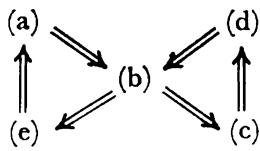
\includegraphics[keepaspectratio]{images/part003_cb91c25e.jpg}}

先证明 (a) 蕴含 (b)；若 A 是因子整环，则 \(P^{*}\) 同构于 A 的除子群，因而同构于 Z 的直和（\(\S\) 1，第3号，定理2）。

注意，现在“两个整主理想的交是主理想”这一关系意味着 A 的每一对元素都有最小公倍元，也就是说 \(P^{*}\) 是格序群（《代数》第VI章，第1节，第9号，命题8）。因此，(b) 蕴含 (c)（事实上与 (c) 等价）这一事实由《代数》第VI章第1节第13号定理2得到。(c) 蕴含 (d) 这一事实由《代数》第VI章第1节第13号命题14（DIV）得到。

(d) 蕴含 (b) 这一事实由《代数》第VI章第1节第13号定理2应用于群 \(\mathcal{P}^*\) 得到。

证明 (b) 蕴含 (e)。若 (b) 成立，则存在从 \(\mathcal{P}^*\) 到 \(\mathbf{Z}^{(I)}\) 的同构；令 \((v_{\iota}(x))_{\iota\in I}\) 表示 \(\mathbf{Z}^{(I)}\) 中与理想 \(Ax\)（\(x\in K^*\)）相对应的元素。显然，每个 \(v_{\iota}\) 都是定义在 \(\mathbf{K}\) 上的离散赋值，\(\mathbf{A}\) 是所有 \(v_{\iota}\) 的赋值环的交，并且对于 \(x\in K^*\)，\(v_{\iota}(x)=0\) 除有限多个指标 \(\iota\) 外成立；所以 \(\mathbf{A}\) 是 Krull 整环。另一方面，设 \(q\) 是 \(\mathbf{A}\) 的高度为1的素理想；它包含一个非零元素 \(a\)，该元素必然不可逆，因而（按素理想的定义）也是某个极值元 \(p\)（属于 \(\mathbf{A}\)）；由于 \(Ap\) 是非零素理想，\(q=Ap\)，这证明 \(q\) 是主理想。

最后证明 (e) 蕴含 (a)。设 \(\mathfrak{a}\) 是 \(\mathbf{A}\) 的除性理想。存在高度为1的素理想 \(p_i\)，它们属于 \(\mathbf{A}\)，使 \(\operatorname{div} \mathfrak{a} = \sum_{i} n_i \operatorname{div} p_i\)，其中 \(n_i \in \mathbf{Z}\)。若 (e) 成立，\(p_i\) 具有 \(A p_i\) 的形式，从而 \(\operatorname{div} \mathfrak{a} = \operatorname{div}\left(\prod_{i} A p_i^{n_i}\right)\)，进而 \(\mathfrak{a} = \prod_{i} A p_i^{n_i}\)，因为 \(\mathfrak{a}\) 是除性理想。

命题1. 设 A 为 Krull 整环。若 A 的每个除性理想都可逆，则对于 A 的每个极大理想 m，\(A_{m}\) 是因子整环。若另加假设 A 的每个除性理想都是有限生成的，则反之亦然（特别地，若 A 是诺特环）。

假设 A 的每个除性理想都可逆；由于 \(A_{m}\) 是 Krull 整环（第1节，第4号，命题6），\(A_{m}\) 的每个除性理想 a 都是两个分式主理想的交（第1节，第5号，命题9的推论2）；所以 \(a = bA_{m}\)，其中 b 是 A 的除性理想（第II章，第2节，第4号）；由于按假设 b 可逆，由第II章第5节第6号定理4可知 a 是主理想，因而 \(A_{m}\) 是因子整环（第1号，定义1）。反过来，若所有 \(A_{m}\) 都是因子整环，且 c 是 A 的有限生成除性理想，则 \(cA_{m}\) 是 \(A_{m}\) 的除性理想，这由第1节第5号命题9的推论2和第II章第2节第4号得到；由假设 \(cA_{m}\) 是主理想，因而由第II章第5节第6号定理4可知 c 可逆。

\subsection{极值元分解}

设 A 为整环，K 为其分式域，U 为 A 的可逆元素乘法群。回忆（《代数》第VI章，第1节，第5号），存在从 \(\mathbf{K}^* / \mathbf{U}\) 到 A 的非零分式主理想群 \(\mathcal{P}^*\) 的典范同构。定理1的条件 (b) 可翻译如下：

命题2. 设 A 为整环。A 为因子整环的充要条件是，存在 A 的子集 P，使 A 的每个 \(a \in A - \{0\}\) 都能唯一写成 \(a = u \prod_{p \in P} p^{n(p)}\)，其中 \(u \in U\)，且 \(n(p)\) 是除有限多个外为零的正整数。

若 P 满足此条件，显然它的所有元素都是极值元，且 A 的每个极值元都与 P 中唯一的一个元素相伴。回忆，P 此时称为 A 的极值元代表系（《代数》第VII章，第1节，第3号，定义2）。

始终假设 A 是因子整环。已经看到（第2节，定理1），群 \(\mathcal{P}^*\) 是一个格。因此可以应用《代数》第VI章第1节第9号和第13号的结果。特别地，\(\mathbf{K}^*\) 中的每个元素都可以以不可约分式的形式，按照本质唯一的方式写出。任意两个
元素 \(a, b\) 属于 \(\mathbf{K}^*\)，都有最大公因元和最小公倍元；若 \(a = u\prod_{p\in \mathbb{P}}p^{n(p)}\)，且

\[
b = u ^ {\prime} \prod_ {p \in P} p ^ {m (p)}
\]

这是 \(a\) 和 \(b\) 作为极值元乘积的分解。于是：

\begin{enumerate}
\def\labelenumi{(\arabic{enumi})}
\tightlist
\item
\end{enumerate}

\[
\mathbf {g . c . d .} (a, b) = w \prod_ {p \in P} p ^ {\inf (m (p), n (p))}\tag{2}
\]

\[
\mathbf {l . c . m .} (a, b) = w ^ {\prime} \prod_ {p \in P} p ^ {\sup (m (p), n (p))}
\]

其中 \(w, w'\) 属于 U。我们特别得到《代数》第VII章第1节第3号的结果。

对于所有 \(p \in P\)，映射 \(a \mapsto n(p)\) 是 K 上的离散赋值 \(v_{p}\)，其赋值环为 \(A_{Ap}\)。由定理1(e) 可知，\(v_{p}\) 正是 A 的本性赋值，而理想 \(A_{p}\)（\(p \in P\)）正是 A 的高度为1的素理想。

\subsection{因子整环的分式环}

命题3. 设 A 为 Krull 整环，S 为 A 的一个不含 0 的乘法子集。

\begin{enumerate}
\def\labelenumi{(\roman{enumi})}
\item
  若 \(\mathbf{A}\) 是因子整环，则 \(\mathbf{S}^{-1}\mathbf{A}\) 是因子整环。
\item
  若 S 由一族元素 \(p_{\iota}\) 生成，且主理想 \(Ap_{\iota}\) 是素理想，并且 \(S^{-1}A\) 是因子整环，则 A 是因子整环。
\end{enumerate}

这立即由第1号定义和第1节第10号命题17得到。

\subsection{因子整环上的多项式环}

设 A 为因子整环，K 为其分式域，f 为 K{[}X{]} 中的非零元素；K* 中的元素 c 若是 f 的系数的最大公因元，则称为 f 的容度。设 v 是 K 上对 A 为本性的赋值，\(\bar{v}\) 是它到 K{[}X{]} 的典范延拓（定义为 \(\bar{v}\left(\sum_{i}a_{i}X^{i}\right)=\inf v(a_{i})\)；参见第VI章第10节第1号命题2）；则 \(\bar{v}(f)=v(c)\)。

引理1（高斯）. 设 \(f, f'\) 是 \(\mathbf{K}[\mathbf{X}]\) 中的非零元素，\(c, c'\) 是 \(f, f'\) 的容度。则 \(cc'\) 是 \(ff'\) 的一个容度。

设 \(d\) 是 \(ff'\) 的容度。对于每个赋值 \(v\)，它定义在 \(K\) 上且对 \(A\) 为本性，令 \(\bar{v}\) 表示它到 \(K[X]\) 的典范延拓。则

\[
v (d) = \bar {v} (f f ^ {\prime}) = \bar {v} (f) + \bar {v} (f ^ {\prime}) = v (c) + v (c ^ {\prime}) = v (c c ^ {\prime}).
\]

因此 \(cc'd^{-1}\) 是 A 的可逆元素。

定理2. 设 A 为因子整环，K 为其分式域，\((p_{\iota})\) 为 A 的极值元代表系，\((\mathrm{P}_{\lambda})\) 为 K{[}X{]} 中不可约多项式的代表系，且每个 \(P_{\lambda}\) 的容度为1。则：

\begin{enumerate}
\def\labelenumi{(\roman{enumi})}
\item
  A{[}X{]} 是因子整环；
\item
  \(p_{\iota}\) 和 \(P_{\lambda}\) 的集合是 A{[}X{]} 的极值元代表系。
\end{enumerate}

设 \(f\) 是 \(A[X]\) 中的非零元素。在环 \(K[X]f\) 中，f 可以唯一分解为如下形式：

\[
f = a \prod_ {\lambda} \mathrm{P} _ {\lambda} ^ {n (\lambda)} \quad (a \in \mathrm{K} ^ {*}, n (\lambda) \geqslant 0).
\]

引理1表明 \(a\) 是 \(f\) 的容度。因此 \(a \in \mathbf{A}\)。由于 \(\mathbf{A}\) 是因子整环，\(a\) 可以唯一分解为如下形式：

\[
a = u \prod_ {\iota} p _ {\iota} ^ {m (\iota)} \quad (u \text {   invertible   in   A }, m (\iota) \geqslant 0).
\]

于是得到以下分解的存在性和唯一性：

\[
f = u \prod_ {\iota} p _ {\iota} ^ {m (\iota)} \prod_ {\lambda} \mathrm{P} _ {\lambda} ^ {n (\lambda)}.
\]

注意，该定理证明了 A 的每个元素在 A 和 A{[}X{]} 中都有相同的极值元分解。因此，A 的一族元素的最大公因元在 A 和 A{[}X{]} 中相同。

也可以利用第1节第10号命题18证明，A{[}X{]} 是因子整环当且仅当 A 是因子整环。

推论。若 A 是因子整环，则环 A{[}X \(_{1}\) , . . . , X \(_{n}\) {]} 是因子整环。

按 n 归纳论证。

该推论可推广到具有无限族不定元的情形（参见习题2）。

\subsection{因子整环与 Zariski 环}

命题4. 设 A 为 Zariski 环，\(\hat{\mathbf{A}}\) 为其完备化。若 \(\hat{\mathbf{A}}\) 是因子整环，则 A 是因子整环。

这由第1号定义以及第1节第10号命题16得到。

推论。若诺特局部环 A 的完备化是因子整环，则 A 是因子整环。
